\documentclass[12pt]{article}
\usepackage[labelfont=bf]{caption}
\usepackage{amssymb}
\usepackage{amsfonts}
\usepackage{amsmath}
\usepackage[nohead]{geometry}
\usepackage[singlespacing]{setspace}
\usepackage[bottom]{footmisc}
\usepackage{indentfirst}
\usepackage{endnotes}
\usepackage{graphicx}
\usepackage{rotating}
\usepackage{hyperref}
\usepackage{enumitem}
\usepackage{graphics}

% due to Subfloats section in  
% http://en.wikibooks.org/wiki/LaTeX/Floats,_Figures_and_Captions
\usepackage{caption}
\usepackage{subcaption}

\usepackage{float}

\usepackage{array}
\usepackage{longtable}
\usepackage{fullpage}
\usepackage{dcolumn}
\usepackage[flushleft]{threeparttable}
\usepackage{booktabs}
\usepackage[12hr]{datetime}
\usepackage[DIV=16]{typearea}
\usepackage{scrextend,booktabs}
\usepackage{tabulary}
\usepackage{multirow}
\usepackage[font=footnotesize]{caption}

\usepackage{booktabs}
\usepackage{threeparttable}

% due to 
% \usepackage{graphicx}
\usepackage{wrapfig}
\usepackage{lscape}
% \usepackage{rotating}
\usepackage{epstopdf}
\usepackage{color, colortbl}
\usepackage[norule,hang]{footmisc}
\setcounter{MaxMatrixCols}{30}
\newtheorem{theorem}{Theorem}
\newtheorem{acknowledgement}{Acknowledgement}
\newtheorem{algorithm}[theorem]{Algorithm}
\newtheorem{axiom}[theorem]{Axiom}
\newtheorem{case}[theorem]{Case}
\newtheorem{claim}[theorem]{Claim}
\newtheorem{conclusion}[theorem]{Conclusion}
\newtheorem{condition}[theorem]{Condition}
\newtheorem{conjecture}[theorem]{Conjecture}
\newtheorem{corollary}[theorem]{Corollary}
\newtheorem{criterion}[theorem]{Criterion}
\newtheorem{definition}[theorem]{Definition}
\newtheorem{example}[theorem]{Example}
\newtheorem{exercise}[theorem]{Exercise}
\newtheorem{lemma}[theorem]{Lemma}
\newtheorem{notation}[theorem]{Notation}
\newtheorem{problem}[theorem]{Problem}
\newtheorem{proposition}{Proposition}
\newtheorem{remark}[theorem]{Remark}
\newtheorem{solution}[theorem]{Solution}
\newtheorem{summary}[theorem]{Summary}
\newenvironment{proof}[1][Proof]{\noindent\textbf{#1.} }{\ \rule{0.5em}{0.5em}}
\makeatletter
\def\@biblabel#1{\hspace*{-\labelsep}}
\makeatother
\geometry{left=1in,right=1in,top=1.00in,bottom=1.0in}
\setlength{\parskip}{0.5em} 
\setlength{\footnotesep}{0.5em}

% \definecolor{name}{system}{definition}
\definecolor{Gray}{gray}{0.9}
\definecolor{LightCyan}{rgb}{0.88,1,1}
\definecolor{PaleGreen}{rgb}{0.807843137,1,0.807843137}
\definecolor{NavajoWhite}{rgb}{1,0.870588235,0.678431373}
\definecolor{Yellow}{rgb}{1,1,0}
\usepackage{lipsum}
\newenvironment{bottompar}{\par\vspace*{\fill}}{\clearpage}


\begin{document}

\title{Unraveling a secret: Vietnam's outstanding performance on the PISA test 2012}
\author{Suhas D. Parandekar
\\Elisabeth K. Sedmik\medskip\\
{\normalsize Global Practice for Education, The World Bank\thanks{E-mail for correspondence: \textit{esedmik@worldbank.org}  This paper has been written using open source software: R for the econometric analysis and graphics and LaTeX for typesetting. Thanks to all who make free software possible and to OECD for making the PISA data freely and easily available to anyone. The R and Latex code used in writing this paper is freely available for download at \href{http://github.com/zagamog/PISA_PAPER}{http://github.com/zagamog/PISA\_PAPER}. The authors would like to thank World Bank colleagues Amer Hasan, Marguerite Clarke, and Thanh Thi Mai for reading earlier versions of the paper and providing helpful feedback. Errors and omissions are the responsibility only of the authors.}} 
\date{\normalsize Date of this draft: \today }}
\maketitle

\sloppy

\textbf{Abstract:} This paper seeks to find an empirical explanation of Vietnam's outstanding performance on the PISA assessment in 2012. Only a few developing countries participate in PISA. Those who do, with the unique exception of Vietnam, are typically clustered at the lower end of the range of PISA scores. This paper compares PISA performance for Vietnam with a set of seven developing countries from the PISA 2012 data set, using a cut-off per capita GDP (in 2010 PPP dollars) of \$10,000. The seven developing countries' average PISA performance lags Vietnam's by more than 100 points. The `Vietnam effect' is difficult to unscramble, but the paper is able to explain about half of the gap between Vietnam and the seven countries. The analysis reveals that Vietnamese students may be approaching their studies with higher diligence and discipline, their parents may have higher expectations, and the parents may be following up with teachers regarding those expectations. The teachers themselves may be working in a more disciplined environment, with tabs being kept on their own performance as teachers. Vietnam may also be benefiting from investments in pre-school education and in school infrastructure that are disproportionately higher when compared to Vietnam's per capita income level. 

\textbf{Keywords:} PISA;Vietnam;Oaxaca-Blinder Decomposition; Fryer-Levitt; Economics of Education.

\textbf{JEL Classification Numbers:} I21 (Analysis of Education); I28(Government Policy); Z18(Public Policy).

%\pagebreak%
\onehalfspacing
%\doublespacing

\section{Introduction}
Vietnam participated in PISA for the first time in 2012 and its performance has been much higher than other developing countries that take part in this OECD led initiative. PISA scores of 15 year-olds in Mathematics, Reading and Science are calibrated to an OECD mean of 500 and standard deviation of 100 points. Only a few developing countries take part in PISA, perhaps because most of them have results much lower than the OECD countries. In the OECD-PISA 2012 database, there are seven countries other than Vietnam with a per capita GDP (in 2010 PPP dollars) below US\$ 10,000 - Albania, Colombia, Indonesia, Jordan, Peru, Thailand and Tunisia. At US\$ 4098, Vietnam's GDP per capita is the lowest of this group. Figure 1 indicates a positive, albeit non-linear correlation between GDP per capita and PISA test scores. Vietnam, represented by a red star, lies much above the other developing countries clustered in the lower left hand corner of Figure 1. With a mathematics mean score of 511, Vietnam is more aligned to Finland (519) and Switzerland (531), rather than Peru (368) and Colombia (376). 
\begin{figure}[H]
   \caption{\textbf{PISA 2012 results compared with GDP per capita}}
   \centering 
     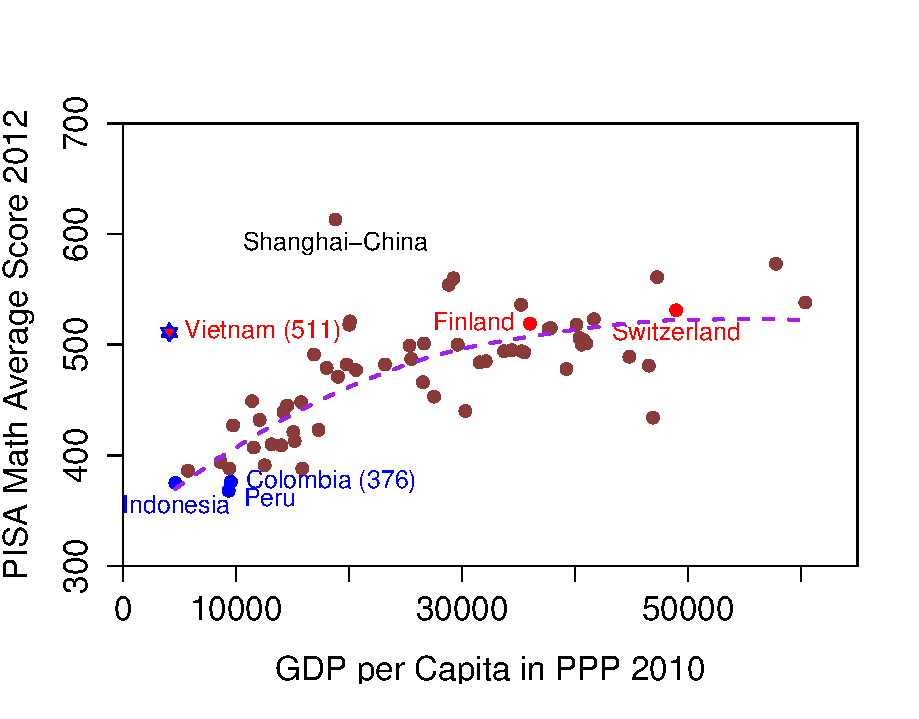
\includegraphics[width=0.75 \textwidth]{INTRFIG1.pdf} \\
\scriptsize{Source: OECD-PISA database        \hspace{3in}     }
   \label{Figure 1} 
\end{figure}
The weighted average mathematics score of the seven developing countries is 383.
It is helpful to understand the significance of the 128 point difference of the seven countries as compared with Vietnam. According to a recent OECD publication \cite{OECD2013a}, \emph{``an entire proficiency level in mathematics spans about 70 score points \textendash  
a large difference in the skills and 
knowledge students at that level possess. Such a gap represents the equivalent of about two years of schooling in the typical OECD country.''} Applying this heuristic would imply a nearly 3 year difference in educational attainment between Vietnam and the group of seven developing countries in the PISA database. It should be noted at the outset that cross-section data from one application of PISA does not permit causal inference, but correlations can still provide useful insights. The difference is not only for mathematics and not just in the mean score, but spanning the entire test distribution, as can be seen in Figure 2.

\begin{figure}[H]
\caption{\textbf{Kernel Density comparison between Vietnam and other Developing Countries}}\label{fig:Kernel}
         \centering
         \begin{subfigure}[b]{0.3\textwidth}
                 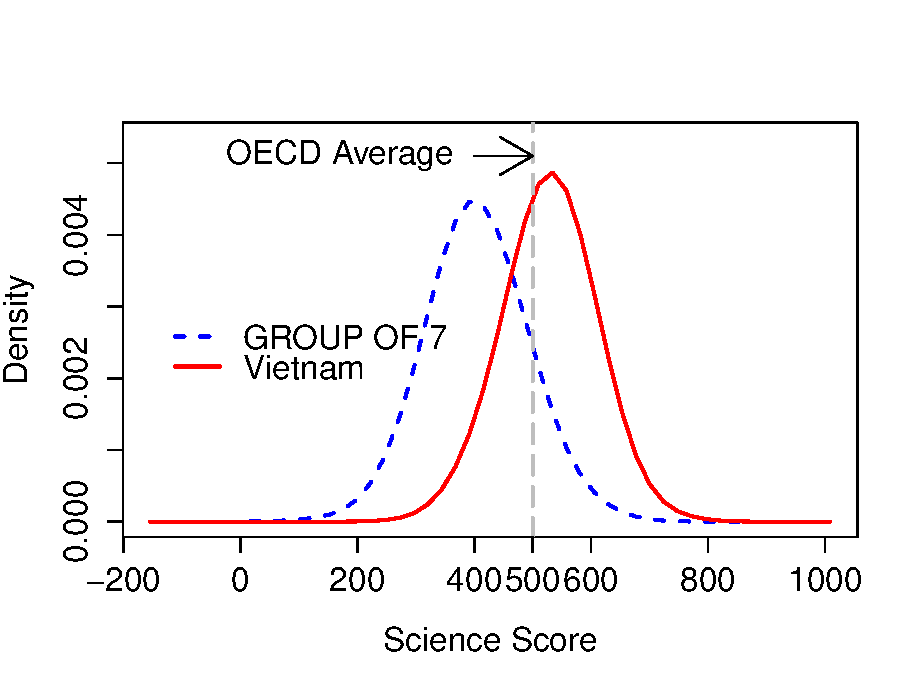
\includegraphics[width=\textwidth]{INTRFIG2a.pdf}
                 \caption{Science}
                 \label{fig:science}
         \end{subfigure}%
         ~ %add desired spacing between images, e. g. ~, \quad, \qquad, \hfill etc.
           %(or a blank line to force the subfigure onto a new line)
         \begin{subfigure}[b]{0.3\textwidth}
                 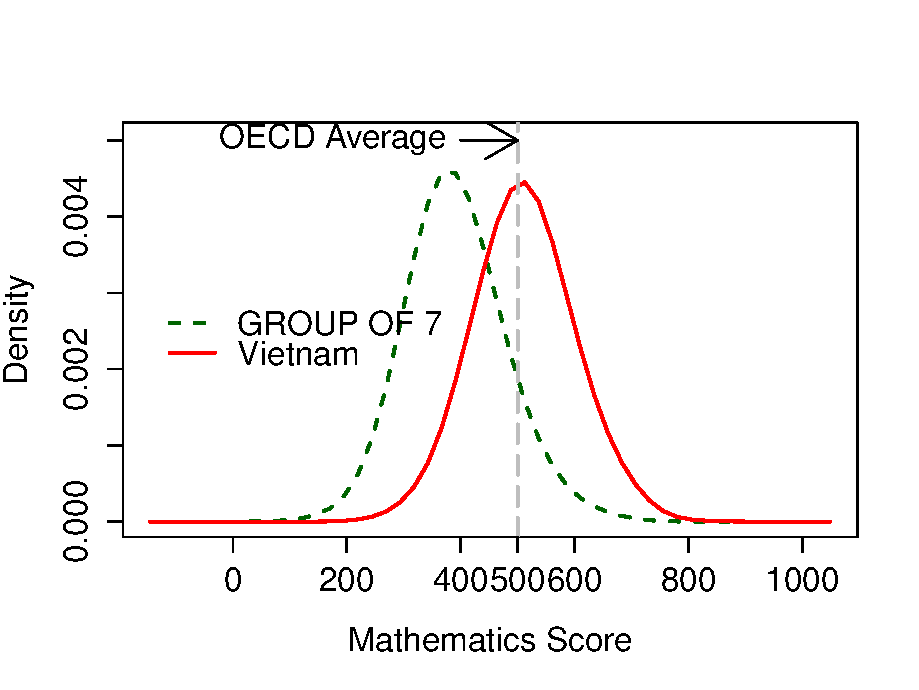
\includegraphics[width=\textwidth]{INTRFIG2b.pdf}
                 \caption{Mathematics}
                 \label{fig:mathematics}
         \end{subfigure}
         ~ %add desired spacing between images, e. g. ~, \quad, \qquad, \hfill etc.
           %(or a blank line to force the subfigure onto a new line)
         \begin{subfigure}[b]{0.28\textwidth}
                 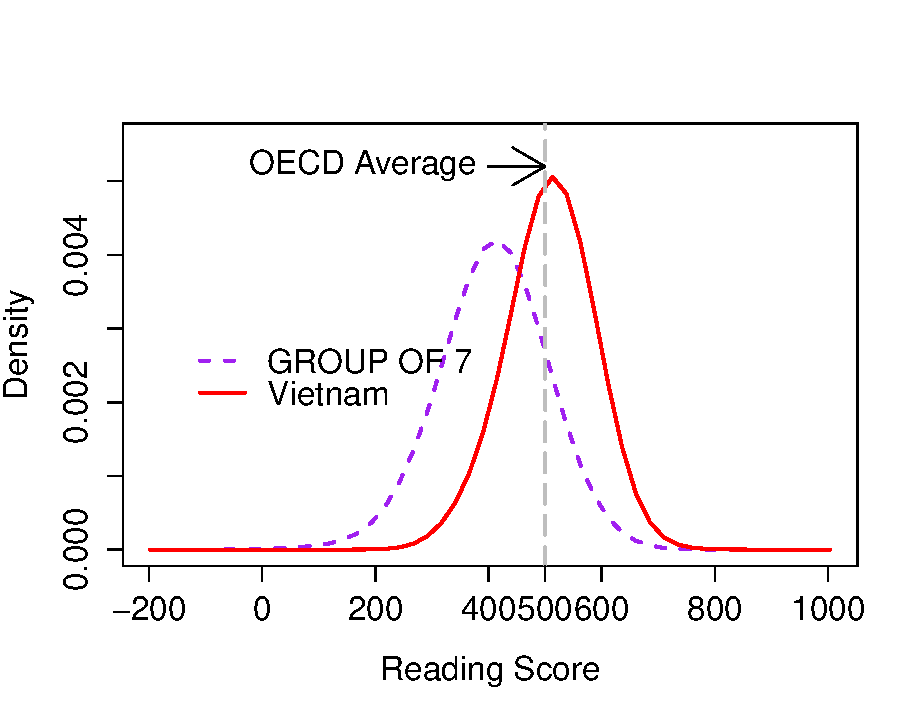
\includegraphics[width=\textwidth]{INTRFIG2c.pdf}
                 \caption{Reading}
                 \label{fig:reading}
         \end{subfigure}
     \end{figure} 

A range of alternative classifications are possible to organize the explanatory factors available in the OECD-PISA database. Figure 3 presents four sets of factors, starting clockwise from the right. This is admittedly an arbitrary classification, utilized merely for expository purposes as we consider each of the constituent variables in turn.

\begin{figure}[H]
	\caption{\textbf{Conceptual Scheme based on available comparative variables}}
	\centering 
	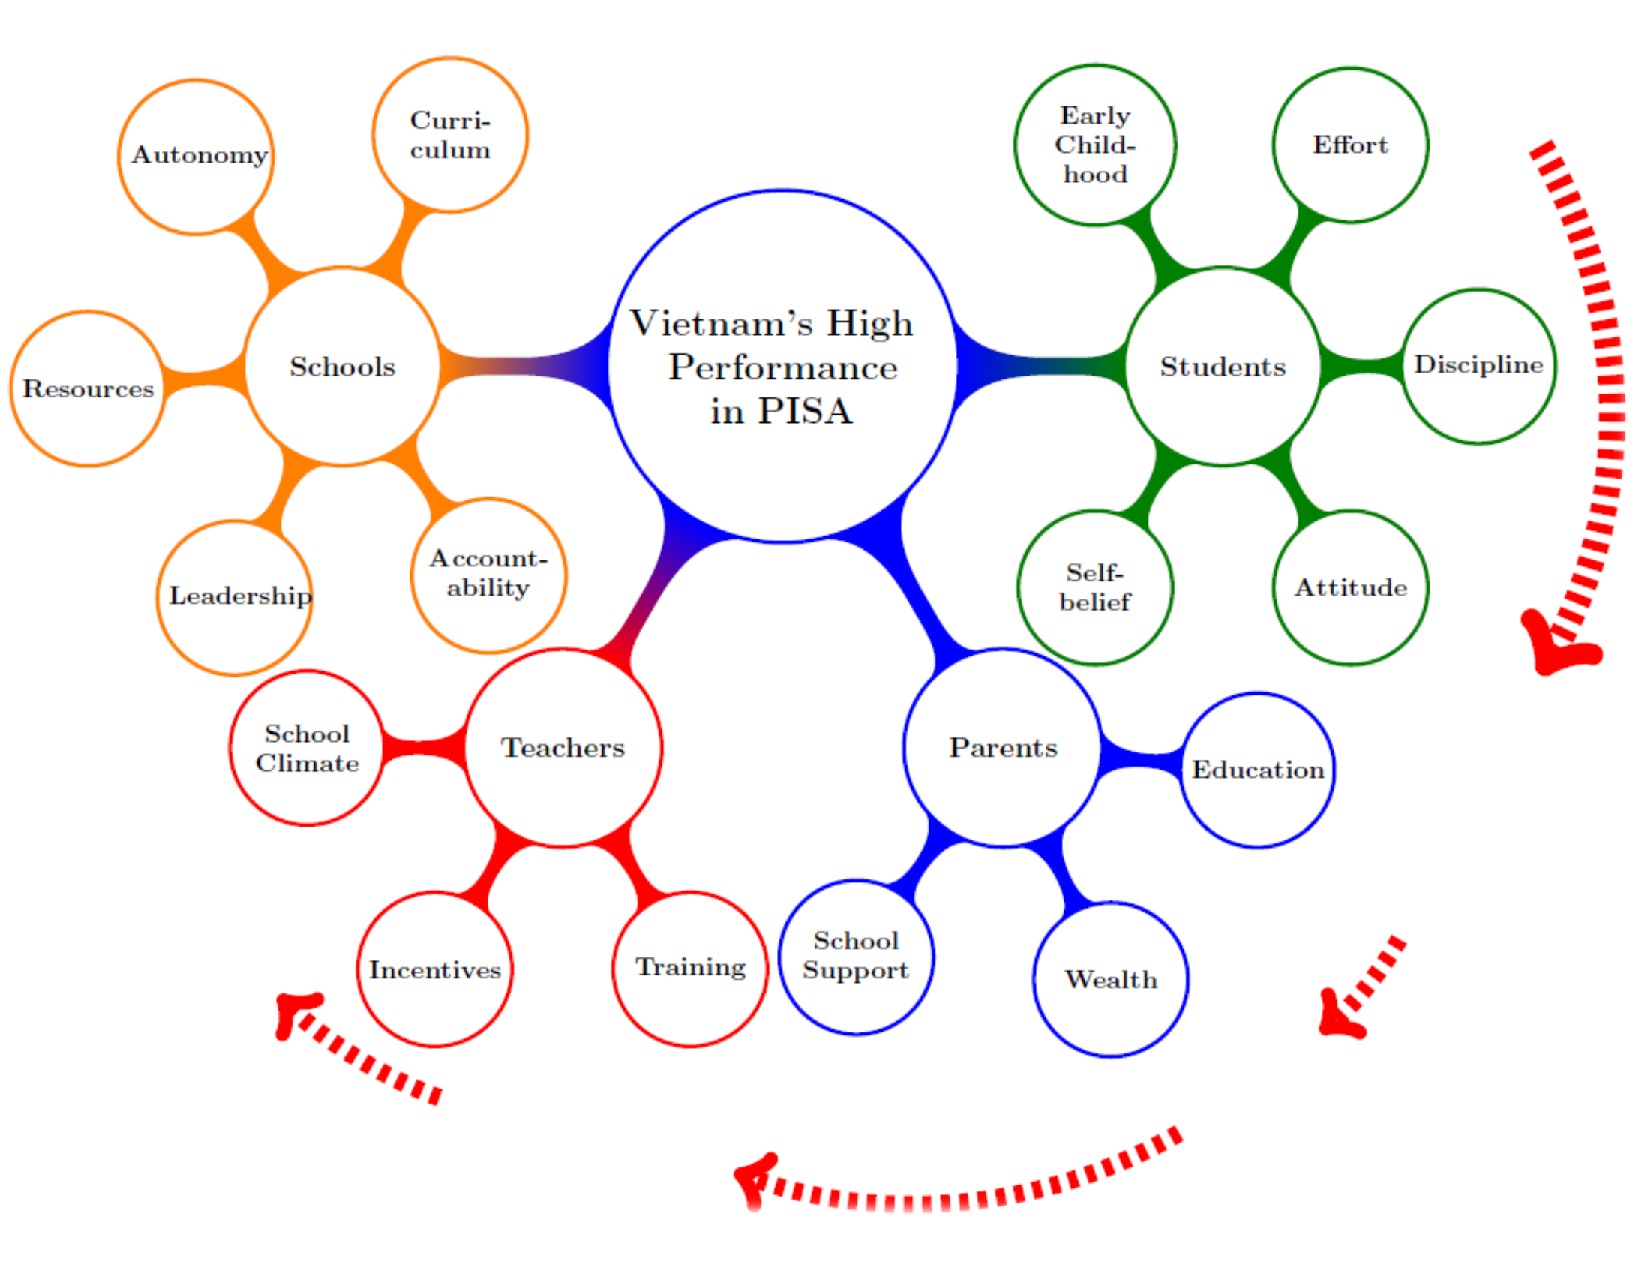
\includegraphics[width = 4.5in]{INTRTIKZ.pdf} 
	\label{fig:m} 
\end{figure}

The approach of this paper is as follows. We begin in Section 2 by examining closely the mean differences between Vietnam and the collective group of seven developing countries, termed as ``Dev7'' for this paper (not to be confused with the G-7 of wealthy countries). Comparing means in this context is a first pass at understanding the performance anomaly of Vietnam on empirical grounds. Do Vietnamese 15 year olds somehow enjoy better cultural, social or civic endowments to balance their economic disadvantages? An examination of mean differences will provide us with a first set of tentative hypotheses.
\par
The insights provided by mean differences need to be explored further by a regression of the test scores on the explanatory variables. Large differences in means may not amount to much if the associated variables are not correlated with test scores. In Section 3 we adopt the regression methodology used by Fryer and Levitt to understand differences in test score results of black children in the first two years of schooling in the United States \cite{FryerLevitt04}. Fryer and Levitt are able to explain away all of a 0.62 standard deviation negative achievement gap for black kindergarten children. In our case, we are able to explain about half of a larger 1.28 standard deviaton  positive achievement gap for Vietnam compared to Dev7 countries. The lower ability of the Fryer-Levitt method to explain the ``Vietnam gap'' is probably accounted for by the fact that per capita GDP lower than US \$ 10,000 is the only common support across diverse economic, political and educational systems.

The Fryer-Levitt method deepens the understanding from mean comparisons, but what it does not reveal may be as interesting as what it does. Our Fryer-Levitt adaption is based on a pooled regression of eight developing countries, where we follow the fate of the magnitude of the coefficient of the dummy variable representing the Vietnamese students in the sample. However, we also need to investigate structural differences in the effects of endowments between Vietnam and Dev7 countries. In Section 4, we adopt an approach first used to explain variation in PISA performance between Germany and Finland by Andreas Ammermueller \cite{Ammermueller07}. This is an adaptation of the popular Oaxaca-Blinder decomposition of wage earnings equation to uncover evidence of discrimination on the basis of gender \cite{Blinder73} and \cite{Oaxaca73}. In this section, we examine closely the structural differences between Vietnam and the Dev7 countries, including the contribution of differences in endowments and the coefficients to the gap in test scores. 

Even a multi-variate regression approach only proves correlation with nothing more than a hint regarding causation, and so far we have only one year (2012) of PISA data for Vietnam. Even though we cannot uncover causality, there are useful policy related conclusions that we can derive from the analysis presented in this paper. There is a veritable industry of papers regarding Finland's PISA performance, directed mostly toward other OECD countries with lower scores, for instance the United States. Vietnam's superlative performance points to a similar future stream of research, with the added advantage of relevance for developing countries. Section 5 provides concluding ideas that might be amongst the first of many more such ideas for future investigations of Vietnam's performance. 

\section{Endowment Differences}

Utilizing the categorization of explanatory factors presented in Figure 3, this section analyzes mean differences in explanatory factors on students, parents, teachers and schools. All variable means presented in the tables are statistically different at the 95\% significance level, unless otherwise noted in the footnotes and figures in parentheses represent standard deviations. PISA documentation, especially the technical report - \cite{OECD2014a} provides rich definitions and explanations of the variables used. Appendix tables A2, A3 and A4 of this paper accordingly provide references mapping the variables used in this paper and the original PISA variable names.

\subsection{Student Characteristics}

Table 1 begins an exploration of differences in mean values between Vietnamese and Dev7 student characteristics. The absence of differences is sometimes as important as the presence of differences. Table 1 indicates no differences by age or gender of students. The PRESCHOOL variable shows the first instance of a large statistically significant difference. While 78.88\% of Dev7 students reported attending pre-school, the number of students attending pre-school from the Vietnam sample was 91.20\% - a sizable difference that is both statistically and economically significant. The relationship between pre-school and later educational outcomes has been studied very closely over the years. Longitudinal impact evaluation studies regarding the Perry Pre-school project and Head Start in the US are amongst the most cited studies in the economics literature\footnote{For detailed meta-analysis, see \cite{Barnett95} and \cite{Schweinhartetal05}}. We can also see from the numbers of REPEAT in Table 1 that PISA takers in Vietnam were three times less likely to have repeated a grade in the past (6.79\% compared to 19.15\%).

\begin{table}[H]
	\tiny
	\def\arraystretch{0.9}
	\centering
	\caption{\textbf{Student characteristics and family background}}
	\begin{threeparttable}	
	\begin{tabulary}{1.0\textwidth}{L L C C C C}
		\hline\hline \\
		\multicolumn{2}{c}{}
		& \multicolumn{2}{c}{Dev7 countries}
		& \multicolumn{2}{c}{Vietnam}	\\
		\hline & & & & & & 
		Variable & Description & MS & Valid N &  MS & Valid N \\
		\hline \\
		\multicolumn{6}{l}{\textbf{Fixed characteristics}}	\\ [0.3em]
      \hline \\
		FEMALE & Sex of student & 0.5265 & 41394 & 0.5336 & 4882 \\ 
		& & (0.4993) &  & (0.4989) &  \\ [0.3em]
      AGE & Age of student & 15.8211 & 41394 & 15.7692 & 4853 \\ 
		& & (0.2895) &  & (0.2885) &  \\ [0.3em]
     \hline \\
     \multicolumn{6}{l}{\textbf{Student's prior history}}	\\ [0.3em]
     \hline \\ 
		PRESCHOOL & Attended Preschool & 0.7888 & 40114 & 0.912 & 4866 \\ 
		&  & (0.4082) &  & (0.2833) &  \\ 
		REPEAT & Grade repeating & 0.1915 & 40343 & 0.0679 & 4860 \\ 
		& &  (0.3935) &  & (0.2516) &  \\ [0.3em]
     \hline \\
     \multicolumn{6}{l}{\textbf{Truancy from School}}	\\ [0.3em]
     \hline \\ 
		ST08Q01 & Times late & 1.5131 & 40663 & 1.1872 & 4873 \\ 
		& for school & (0.7648) &  & (0.4685) &  \\ [0.3em]
		ST09Q01 & Days unexcused & 1.2192 & 40650 & 1.0999 & 4875 \\ 
		& absence & (0.5276) &  & (0.3527) &  \\ [0.3em]
		ST115Q01 & Times skipped & 1.2585 & 40632 & 1.0764 & 4880 \\ 
		& classes & (0.545) &  & (0.3216) &  \\ [0.3em]
     \hline \\
     \multicolumn{6}{l}{\textbf{Parental background and family wealth}}	\\ [0.3em]
     \hline \\ 
		HISEI & Highest parental & 40.4196 & 32814  & 26.6023 & 4860 \\ 
		& occupational status & (22.5168) &  & (19.855) &  \\ [0.3em]
		MISCED & Educational level & 3.1193 & 40486 & 2.1744 & 4844 \\ 
		& of mother (ISCED) & (1.9853) &  & (1.6059) &  \\ [0.3em]
		WEALTH & Family wealth & -1.4606 & 40821 & -2.1343 & 4881 \\ 
		& possessions & (1.2267) &  & (1.1656) &  \\ [0.3em]
		CULTPOS & Cultural possessions & -0.1424 & 39905 & -0.2361 & 4809 \\ 
		& & (0.9678) &  & (1.0173) &  \\ [0.3em]
		HEDRES & Home educational &  -0.7427 & 40579 & -1.0743 & 4874 \\ 
		& resources & (1.1473) &  & (0.9364) &  \\ [0.3em]
		BOOK\_N & Number of books & 53.6393 & 39631 & 50.786 & 4841 \\ 
		& in family home & (94.5556) &  & (75.4031) &  \\[0.3em]
		\hline
		\end{tabulary}
		\begin{tablenotes}[para,flushleft]
		Notes: The variables relate to the questionnaires administered to students in the general  
		(non-rotated) booklet. For a more detailed description of variables, please see Tables A2, A3, A4 in the Appendix.The variable means of Dev7 and Vietnam are statistically different at the 95\% significance level,
		except FEMALE. Figures in parenthesis represent standard deviations. 
		\end{tablenotes}
		\end{threeparttable}
\end{table}
The findings regarding PRESCHOOL and REPEAT indicates the possible importance of the trajectory of the student prior to High School. Repetition rates are difficult as comparative indicators of system quality because of the variations across countries in curriculum and standards, but REPEAT is another interesting variable to keep in mind as a possible clue to the mystery of Vietnam's PISA performance. As in some other East Asian cultures, Vietnamese parents expect their children to study hard. Though Mark Twain, translated into Vietnamese is quite a best seller for young readers in Vietnam, truancy from school is not perceived benevolently by parents.\footnote{A cultural explanation is possibly quite important in explaining Vietnam's anomalous PISA results, though the PISA dataset may only be able to measure the possible effects of culture rather than measuring cultural differences. Literature from the World Values Survey, that does seek to measure cultural differences, indicates that Vietnam is a positive outlier on discipline and authority orientation\cite{DaltonOng05}.} Table 1 indicates a consistently lower truancy rate for the three variables used.  The question refers to the past two complete weeks of school and we can see that Vietnamese students are less likely to have been late for school, have fewer days of unexcused absence and skip fewer classes.\footnote{In the student's questionnaire, there is a telling question - student's have to agree or disagree on a four point Likert scale to the statement ``If I had different teachers, I would try harder at school.''. Converted into an index, the mean for Vietnam at 0.363 is lower than that for Dev7 at 0.525. This suggests a tendency in Vietnamese students for greater self-responsibility.} 

The final set of variables in Table 1 concerns parental background and wealth at the students home, including cultural resources and books at home which may work to stimulate cognitive development. The PISA database includes a number of indices to measure aspects such as wealth. These indices are based on underlying data regarding occupations and possessions. The scaling of raw data to indices is described in detail in the PISA technical report \cite{OECD2014a}. For HISEI, which describes parental occupation status, the OECD mean is 50 and the OECD standard deviation is 15. Table 1 shows that HISEI for Dev7 parents stands at 40.42 and is thus much higher than 26.60 for Vietnamese parents. MISCED refers to the International Standard Classification of Education (ISCED) developed by UNESCO. Table 1 shows that the average level of mother's education (MISCED) for Dev7 was just over 3, meaning Upper Secondary education, while for Vietnam the mean was just over 2, meaning Lower Secondary education. The WEALTH index is set for an OECD mean of zero and standard deviation of 1. Dev 7 countries wealth level was -1.5 and Vietnam's was -2.1, which is consistent with the data regarding occupational classification and mother's education. These findings indicate the close correlation of these variables with GDP per capita. Another interesting finding concerns the indices CULTPOS, cultural possessions and HEDRES, educational resources at home which have an OECD mean 0 and a standard deviation 1, as well as BOOK\_N, the number of books in family home. CULTPOS includes classical literature, books of poetry and works of art. HEDRES includes reference books and books to help with school work as well as a study desk and ``a quiet place to study''. These three variables are also in line with per capita income - with the Dev7 mean being lower than the OECD mean, and Vietnam being lower than the Dev7 mean. One explanation regarding Vietnam's PISA performance can probably be ruled out - it does not seem likely that Vietnamese households spend a disproportionately higher amount of their income on acquiring possessions such as books and other objects that would give their children an edge in life.

\subsection{Student Effort}

The phenomenon of primary and high school children taking extra classes to supplement in-school instruction in Vietnam is well known, see \cite{HaHapharm05} and \cite{Hai-Anh07}. Table 2 indicates that while Dev7 students spent roughly 4.7 hours in such classes (total of OUTMATH, OUTLANG and OUTSCIE), the Vietnamese student spends nearly 2 hours more for a total of 6.6 hours per week in such classes, with the difference being highest for OUTMATH. Vietnamese students also spent about 1 additional hour per week doing homework (total of ST57Q01 and ST57Q02) compared to Dev7 students. The highest difference in this set of variables concerns the variable ST57Q04, which relates to extra classes taught by a commercial company. While most of the schools in Vietnam are public or government schools, it is interesting to note that students report nearly 5 hours of commercially provided extra lessons, while the total for Dev7 countries is only about 2 hours per week. Collectively, these variables indicate that Vietnamese students spent about 16 hours per week studying outside of school, compared to 13 hours per week for Dev7 students. 

\begin{table}[H]
	\tiny
	\def\arraystretch{0.9}
	\centering
	\caption{\textbf{Student studying time out of school}}
	\begin{threeparttable}	
	\begin{tabulary}{1.0\textwidth}{L L C C C C}
		\hline\hline \\
		\multicolumn{2}{c}{}
		& \multicolumn{2}{c}{Dev7 countries}
		& \multicolumn{2}{c}{Vietnam}	\\
		\hline & & & & & & 
		Variable & Description & MS & Valid N &  MS & Valid N \\
		\hline \\
\multicolumn{6}{l}{\textbf{Weekly out-of-school hours per subject}}	\\ [0.3em]
\hline \\
OUTMATH \textit{(r)}& weekly out-of-school & 1.828 & 23603 & 3.1305 & 3227 \\ 
& lessons in math & (2.1539) &  & (2.3133) &  \\ [0.3em]
OUTREAD \textit{(r)}& weekly out-of-school & 1.2882 & 23531 & 1.4483 & 3223 \\ 
& lessons in 'test language'& (1.9623) &  & (1.8837) &  \\ [0.3em]
OUTSCIE \textit{(r)} & weekly out-of-school & 1.5609 & 23298 & 2.0927 & 3205 \\ 
& lessons in science & (2.0456) &  & (2.1776) &  \\ [0.3em]
\hline \\
\multicolumn{6}{l}{\textbf{Weekly out-of-school hours approach}}	\\ [0.3em]
\hline \\
ST57Q01 \textit{(r)} & Out-of-school time & 5.0953 & 23696 & 5.8145 & 3164 \\ 
& homework & (5.0319) &  & (5.7196) &  \\ [0.3em]
ST57Q02 \textit{(r)} & Out-of-school time & 2.551 & 19355 & 2.8814 & 2285 \\ 
& guided homework & (2.9296) &  & (3.2384) &  \\ [0.3em]
ST57Q03 \textit{(r)} & Out-of-school time & 1.7276 & 20367 & 1.5749 & 3049 \\ 
& personal tutor & (2.7884) &  & (2.938) &  \\[0.3em]
ST57Q04 \textit{(r)} & Out-of-school time & 1.892 & 19517 & 4.878 & 3091 \\ 
& classes by company & (3.3487) &  & (4.8058) &  \\ [0.3em]
ST57Q05 \textit{(r)} & Out-of-school time & 2.1354 & 21542 & 1.7646 & 3092 \\ 
& parent/family member & (3.055) &  & (3.2442) &  \\ [0.3em]
ST57Q06 \textit{(r)} & Out-of-school time & 2.588 & 21338 & 1.8029 & 3079 \\ 
& learn on computer & (3.5519) &  & (3.0496) &  \\ [0.3em]
		\hline
\end{tabulary}
\begin{tablenotes}[para,flushleft]
		Notes: The variables relate to the questionnaires administered to students in the rotated  
		booklet, marked with \textit{(r)}. For a more detailed description of variables, please see Tables A2, A3, A4 in the Appendix. The variable means of Dev7 and Vietnam are statistically different at the 95\% significance level. Figures in parenthesis represent standard deviations. 		
\end{tablenotes}
\end{threeparttable}
\end{table}

\subsection{Student Attitudes}

PISA applications in each test round have a focus on one of the subjects and in PISA 2012 the focus subject was mathematics. Mathematics happens to be the subject where the mean score difference is highest between Vietnam and Dev7 countries. The PISA questionnaire for students includes a very interesting series of questions regarding students' perceptions of their abilities, their effort and their reported practices. The details of these questions can be found in the PISA technical report \cite{OECD2014a}. Typically, each question includes a set of Likert scaled items to which the student provides a discrete response on a four point agree-disagree scale. These responses are then combined under specified algorithms to provide an index value. For instance, MATWKETH, is meant to measure a student's ``mathematics work ethic''. Students either agree or disagree with a set of 9 items on a 4 point likert scale - strongly disagree, disagree, agree and strongly disagree. The items include items such as ``I work hard on my mathematics homework'',  and ``I listen in mathematics class'', ``I keep my mathematics work well organized''. In the case of MATWKETH, when a student agrees/strongly agrees with a positive statement, or disagrees/strongly disagrees with a negative statement, he or she would tend to be deemed to have a stronger work ethic towards mathematics. The raw data from the Likert scale is converted into an index using IRT scaling procedures, so that the mean for OECD countries is 0 and the standard deviation is 1. Table 3 indicates a most interesting finding regarding a range of such indices from the PISA database.

\begin{table}[H]
	\tiny
	\def\arraystretch{0.9}
	\centering
	\caption{\textbf{Student self-perception regarding mathematical ability and student effort}}
	\begin{threeparttable}
	\begin{tabulary}{1.0\textwidth}{L L C C C C}
		\hline\hline \\
		\multicolumn{2}{c}{}
		& \multicolumn{2}{c}{Dev7 countries}
		& \multicolumn{2}{c}{Vietnam}	\\
		\hline & & & & & & 
		Variable & Description & MS & Valid N &  MS & Valid N \\
		\hline \\
	\multicolumn{6}{l}{\textbf{Indices susceptible to 'bragging' tag }}	\\ [0.3em]
	\hline \\		
   MATWKETH \textit{(r)} & Mathematics & 0.4514 & 26140 & -0.0014 & 3217 \\ 
	& work ethic & (0.9782) &  & (0.6915) &  \\ [0.3em]	
	SUBNORM \textit{(r)} & Subjective norms & 0.716 & 26509 & -0.0923 & 3220 \\ 
	& in mathematics & (1.165) &  & (0.8395) &  \\ [0.3em]
	OPENPS \textit{(r)} & Openness to & 0.1949 & 25612 & -0.6125 & 3207 \\ 
	& problem solving & (0.9787) &  & (0.8708) &  \\ [0.3em]
	SCMAT \textit{(r)} & Self-concept of & 0.1673 & 26222 & -0.1896 & 3249 \\ 
	&  own math skills & (0.8101) &  & (0.5903) &  \\ [0.3em]
	\multicolumn{6}{l}{\textbf{Indices less related to bragging/being boastful}}	\\ [0.3em]
	\hline \\		
	PERSEV \textit{(r)} & Perseverance & 0.3387 & 25710 & 0.4475 & 3211 \\ 
	& in problem solving & (0.9605) &  & (0.8767) &  \\ [0.3em]
	ANXMAT \textit{(r)} & Mathematics & 0.3995 & 26275 & 0.2115 & 3248 \\ 
	& Anxiety & (0.7724) &  & (0.6354) &  \\ [0.3em]
	MATINTFC \textit{(r)} & Mathematics & 0.092 & 24827 & 0.3285 & 3181 \\ 
	& intentions & (0.9837) &  & (1.0964) &  \\ [0.3em]
		\hline
		\end{tabulary}
		\begin{tablenotes}[para,flushleft]
		Notes: The variables relate to the questionnaires administered to students in the rotated  
		booklet, marked with \textit{(r)}. For a more detailed description of variables, please see Tables A2, A3, A4 in the Appendix. The variable means of Dev7 and Vietnam are statistically different at the 95\% significance level. Figures in parenthesis represent standard deviations. 
		\end{tablenotes}
		\end{threeparttable}	
\end{table}

The upper panel in Table 3 indicates a set of indices for which the scores of Vietnamese students are lower than the scores of Dev7 students. For example, the score for MATWKETH is 0.45 for Dev7 and 0 for Vietnam. The variable SUBNORM is supposed to measure subjective norms regarding mathematics. This construct relates to a student's perceptions regarding how other people in the student's life value mathematics. It includes items such as ``my friends enjoy taking mathematics tests'' and ``my parents believe it's important for me to study mathematics.'' Presumably, when this measure is high, the student has a high subjective norm for mathematics. Table 3 shows that the resulting mean for Dev7 countries is 0.72 and the corresponding value for Vietnam is -0.09. The index SCMAT includes items such as ``I learn mathematics quickly'' and ``I have always believed that mathematics is one of my best subjects''. Vietnamese students, who scored more than 1 standard deviation above the Dev7 students on the PISA math test, scored half a standard deviation lower on SCMAT. What is going on here?

This mini-mystery within the overall mystery of Vietnam's PISA performance can possibly be resolved by looking at some further indices.  The lower panel of Table 3 reports on indices where the balance tips to the other side - these are indices where Vietnamese students have a higher mean value than Dev7 students. These three indices bear close examination. PERSEV consists of items that purport to capture perseverance with a task or a problem to resolve; ANXMAT is a negative index (less is better) that deals with mathematics anxiety (for example, an item included in this index states that ``I get very nervous doing mathematics problems''); MATINTFC relates to future mathematics intention, including items such as ``I am planning on majoring in a subject in college that requires lots of mathematics''. 

One possible explanation, as indicated in the heading of the Table 3 panels, is that Vietnamese students are brought up in a culture that stresses the importance of modesty and humility as a pathway to learning. They may find it difficult to say great things about themselves, because of cultural norms against bragging or boasting. The lower panel in Table 3, on the other hand includes items that are less prone for an immodest interpretation. To say that you are not afraid of mathematics may not be perceived as bragging. In this context, the Vietnamese students are less anxious and more confident about the future role of mathematics in their life.\footnote{It will be straightforward to examine this hypothesis more closely by performing an IRT scaling of the underlying items for the indices. We can then test for differences between Vietnam and the Dev7 countries in values of the  location parameters linking the items to the index. Systematic differences will tend to support the hypothesis laid out here.}

\subsection{Mathematics Curriculum}

In addition to beliefs and perceptions of students regarding mathematics in general, PISA also seeks to closely investigate the issues related to the content of mathematics instructions. PISA incorporates a very interesting approach to avoid or minimize the bragging or over-claiming problem referred to in the previous sub-section. The index FAMCON is constructed out of a response to a question about mathematical concepts for which students are asked ``How familiar are you with the following items?'' The list of items includes items such as `Linear Equation', `Quadratic Function' and `Cosine.' The list of items also includes three nonsensical items or pseudo-concepts that sound fancy: `Proper Number',`Subjunctive Scaling' and `Declarative Fraction'. These items are termed as ``FOIL'', and are used as trick items to calibrate the response for over-claiming on part of the students. The index without correction is presented as FAMCON, and the index with correction is presented as FAMCONC. It is quite fascinating that with FAMCON, the "uncorrected" version, Dev7 students come out apparently better than Vietnam students, with a mean value of 0.26 as compared to 0.12. Unfortunately, this also included familiarity with non-existent items like `subjunctive scaling' - or bragging. With the corrected version, FAMCONC, the Vietnamese students turn out to do much better, with a mean value of 0.43 as compared -0.54 for Dev7, as can be seen in Table 4. 

\begin{table}[H]
	\tiny
	\def\arraystretch{0.9}
	\centering
	\caption{\textbf{Student reported experience in mathematics}}
	\begin{threeparttable}
	\begin{tabulary}{1.0\textwidth}{L L C C C C}
		\hline\hline \\
		\multicolumn{2}{c}{}
		& \multicolumn{2}{c}{Dev7 countries}
		& \multicolumn{2}{c}{Vietnam}	\\
		\hline & & & & & & 
		Variable & Description & MS & Valid N &  MS & Valid N \\
		\hline \\	
		FAMCON \textit{(r)} & Familiarity with & 0.2559 & 26164 & 0.1225 & 3243 \\ 
		& math concepts & (1.1654) &  & (0.6935) &  \\ 	[0.3em]
		FAMCONC \textit{(r)} & FAMCON corrected & -0.5441 & 25832 & 0.4297 & 3231 \\ 
		& with FOIL & (0.8768) &  & (0.9057) &  \\ 	[0.3em]
		EXAPPLM \textit{(r)} & Experience with & 0.1111 & 26133 & -0.2418 & 3243 \\ 
		& applied math tasks & (1.06) &  & (0.7624) &  \\ [0.3em]
		EXPUREM \textit{(r)} & Experience with pure & -0.1384 & 25973 & 0.1587 & 3244 \\ 
		& math tasks & (0.9809) &  & (0.8076) &  \\ [0.3em]
		\hline
		\end{tabulary}
		\begin{tablenotes}[para,flushleft]
		Notes: The variables relate to the questionnaires administered to students in the rotated  
		booklet, marked with \textit{(r)}. For a more detailed description of variables, please see Tables A2, A3, A4 in the Appendix. The variable means of Dev7 and Vietnam are statistically different at the 95\% significance level. Figures in parenthesis represent standard deviations. 
		\end{tablenotes}
		\end{threeparttable}
\end{table}

The index EXAPPLM asks students about their experience during school work with examples of applied mathematics problems. Similarly, the index EXPUREM refers to experience with examples of pure mathematics. Not surprisingly, Vietnamese students indicate a lower performance on EXAPPLM and a higher performance on EXPUREM.\footnote{It has been a long standing issue that Vietnamese students are expected to learn a curriculum that is more ``crammed'' than the international norm and contains more theory and abstract mathematics rather than applied mathematics. See \cite{NguyenTran13} and \cite{Le07}.} 

\subsection{Parental Support at School} 

The publication of the bestselling book \cite{Chua11} ``Battle Hymn of the Tiger Mother'' in 2011 ignited a firestorm of controversy. The book gave prominence in popular culture to a vast academic literature regarding parenting styles and the perceived higher performance of children from Asian immigrant families in the US and other Western countries. One of the ways that parents influence their children's educational outcome is through the interaction that parents have with their child's teachers and others at school. The PISA data includes a question that tries to examine parental expectations towards schools. The question SC24 includes a statement ``There is \emph{constant pressure} from many parents, who expect our school to set very high academic standards and to have our students achieve them.''\footnote{\cite{HsinXie14} investigate in great detail data from a set of longitudinal surveys that cover thousands of children over a long period of time starting from their early childhood through High school. As part of the explanation of the superior performance of Asian immigrant children, the authors report that ``Asian students report greater parental expectations of academic success.'' }  Table 5 indicates a higher level of PARPRESSURE (an index derived from SC24) for Vietnam, compared to Dev7.  Another question (SC25) asks school principals about the proportion of parents that take part in a set of 12 activities. While the question does not specify which parent (or both) may be involved, the variables, that may contain more than one of these activities, have been named after the mother for ease of exposition. 

\begin{table}[H]
	\tiny
	\def\arraystretch{0.9}
	\centering
	\caption{\textbf{Parental Support at School}}
	\begin{threeparttable}
	\begin{tabulary}{1.0\textwidth}{L L C C C C}
		\hline\hline \\
		\multicolumn{2}{c}{}
		& \multicolumn{2}{c}{Dev7 countries}
		& \multicolumn{2}{c}{Vietnam}	\\
		\hline & & & & & & 
		Variable & Description & MS & Valid N &  MS & Valid N \\
		\hline \\
		PARPRESSURE & Parental achievement & 0.2665 & 40372 & 0.3837 & 4866 \\ 
		& pressure & (0.4421) &  & (0.4863) &  \\  [0.3em]
		TIGERMOM & Parent initiates - &  52.4472 & 41394 & 62.4183 & 4882 \\ 
		& progress discussion & (38.097) &  & (41.3743) &  \\ [0.3em]
		DUTYMOM & Teacher initiates - &  66.9737 & 41394 & 68.5543 & 4882 \\ 
		& progress discussion & (36.727) &  & (37.4796) &  \\ [0.3em]
		VOLUMOM & Parent Participation - & 35.2134 & 41394 & 38.3623 & 4882 \\ 
		& Volunteering & (38.8428) &  & (39.9773) &  \\ [0.3em]
		TEACHMOM & Parent Participation - & 12.1764 & 41394 & 38.2821 & 4882 \\ 
		& Teaching Assistance & (23.4241) &  & (41.5357) &  \\ [0.3em]
		FUNDMOM & Parent Participation - & 23.0784 & 41394 & 59.6022 & 4882 \\ 
		& Fundraising & (35.2134) &  & (44.0376) &  \\ [0.3em]
		COUNCILMOM & Parent Participation - & 36.4546 & 41394 & 23.1174 & 4882 \\ 
		& School government & (37.2252) &  & (36.4406) &  \\[0.3em]
		\hline
		\end{tabulary}
		\begin{tablenotes}[para,flushleft]
		Notes: The variables relate to the questionnaires administered to schools. For a more detailed description of variables, please see Tables A2, A3, A4 in the Appendix. The variable means of Dev7 and Vietnam are statistically different at the 95\% significance level. Figures in parenthesis represent standard deviations. 
		\end{tablenotes}
		\end{threeparttable}
\end{table}

TIGERMOM refers to the reported proportion of parents who discussed their child's behavior or the child's progress ``on their own initiative'', to differentiate from cases where parents might have done so following the initiative of the teacher, termed as DUTYMOM. Table 4 shows a slightly higher number on DUTYMOM for Vietnamese parents compared to Dev7, but a greater difference, more than ten percentage points for TIGERMOM. VOLUMOM refers to parents volunteering in various non-academic activities, such as field trips or carpentry and yard work. Vietnamese parents appear to have a slight advantage with regard to VOLUMOM, yet a much higher one when considering TEACHMOM, which refers to parents volunteering as assistants to the teacher - 38.28\% compared to 12.18\% for Dev7. Vietnamese parents also appear to be much more active in fund raising, looking at FUNDMOM, though they may have less formal influence through school committees. 

\subsection{Teacher Characteristics} 

Conventional measures regarding student-teacher ratios and teacher certification show some advantage for Vietnam over Dev7 as shown in Table 6.  

\begin{table}[H]
	\tiny
	\def\arraystretch{0.9}
	\centering
	\caption{\textbf{Teacher characteristics and management}}
	\begin{threeparttable}
	\begin{tabulary}{1.0\textwidth}{L L C C C C}
		\hline\hline \\
		\multicolumn{2}{c}{}
		& \multicolumn{2}{c}{Dev7 countries}
		& \multicolumn{2}{c}{Vietnam}	\\
		\hline & & & & & & 
		Variable & Description & MS & Valid N &  MS & Valid N \\
		\hline \\
		\multicolumn{6}{l}{\textbf{Teacher numbers and teacher management}}	\\ [0.3em]
		\hline \\ 
		PROPCERT & Proportion of & 0.6757 & 35130 & 0.7961 & 4586 \\ 
		& certified teacher & (0.4042) &  & (0.3978) &  \\ [0.3em]
		SMRATIO & Mathematics & 188.1791 & 33985 & 120.9773 & 4777 \\ 
		& teacher-student ratio & (158.6256) &  & (43.6092) &  \\ [0.3em]
		SC35Q02 & Professional development & 40.5068 & 39550 & 49.0086 & 4762 \\ 
		& in math in last 3 months & (40.8546) &  & (45.1706) &  \\ [0.3em]
		STUDREL \textit{(r)} & Teacher student & 0.3794 & 25870 & 0.0186 & 3253 \\ 
		& relations & (1.0178) &  & (0.8883) &  \\ [0.3em]
		TCH\_INCENTV & Teacher appraisal  &  -0.0317 & 41394 & 0.2687 & 4882 \\ 
		& linked to incentives & (1.0301) &  & (0.6336) &  \\ 	[0.3em]
		\hline \\
		\multicolumn{6}{l}{\textbf{Quality assurance of mathematics teachers through \ldots}}	\\ [0.3em]
		\hline \\ 
		TCH\_MENT & Teacher mentoring & 0.8566 & 40734 & 0.9859 & 4882 \\ 
		& as quality assurance & (0.3505) &  & (0.1181) &  \\ [0.3em]
		TCM\_PEER & Teacher peer review & 0.7916 & 41095 & 0.8382 & 4882 \\ 
		& of lectures, methods etc & (0.4061) &  & (0.3683) &  \\ [0.3em]
		TCM\_OBSER & Principal or senior & 0.8015 & 41170 & 0.9785 & 4882 \\ 
		& staff observations & (0.3989) &  & (0.1451) &  \\ [0.3em]
		TCM\_INSPE & Observation of classes & 0.5882 & 41020 & 0.8664 & 4882 \\ 
		& external inspector & (0.4922) &  & (0.3402) &  \\ [0.3em]
		\hline
		\end{tabulary}
		\begin{tablenotes}[para,flushleft]
		Notes: The variables relate to the questionnaires administered to schools and students in the rotated  
		booklet, marked with \textit{(r)}. For a more detailed description of variables, please see Tables A2, A3, A4 in the Appendix. The variable means of Dev7 and Vietnam are statistically different at the 95\% significance level. Figures in parenthesis represent standard deviations. 
		\end{tablenotes}
		\end{threeparttable}
\end{table}

The overall student-teacher ratio is not much different for Vietnam and Dev7 and stands at roughly 20 students per teacher. However, there are more specialized mathematics teachers per student in Vietnam, as shown by the values for SMRATIO (121 in Vietnam compared to 188 for Dev7). There is a higher percentage of certified teachers in Vietnam and higher reported professional development in mathematics (SC35Q02). A very interesting variable from a policy point of view regards the incentives for teachers. School principals were asked to what extent performance appraisal or other forms of feedback are related to incentives for teachers in seven different forms, from salary and bonus to public recognition and greater job responsibilities. The answers were to be given on a 4 point scale: `No change', `A small change', 'A moderate change' and 'A large change'. We converted the rating into a Rasch index, scaled to an OECD mean of 0 and standard deviation of 1. The mean for Dev7 for this index, TCH\_INCENTV was -0.03 for Dev7 and 0.27 for Vietnam, indicating greater presence of teacher incentives in Vietnam. The final set of variables in Table 6 deal with the way that quality assurance regarding teacher performance is carried out, with help of a mentor, peer, supervisor or external inspector. These variables indicate a higher prevalence of oversight for teachers in Vietnam, with the difference being greatest for external inspections (86.64\% in Vietnam compared to 58.82\% in Dev7 countries). 

\subsection{Pedagogical Practices} 

Pedagogical practices are an outcome of a complex interaction between curriculum and related educational policies, economic possibilities and the cultural and historical context. It is difficult to trace differences in these practices in a quantitative survey.\footnote{For an interesting recent qualitative study that seeks to emulate the TIMSS video study for Vietnam, see \cite{Phuong14}.} Table 7 presents a few variables that seek to capture variation in pedagogical practices. They indicate the higher prevalence of national policies in Vietnam regarding the use of computers in the classroom and the use of a standardized curriculum that specifies what has to be taught each month. There is no difference with regard to the use of a single textbook. There is some difference in the use of formative student assessment, with slightly higher percentage of use of assessments to monitor teachers and schools in Vietnam. COGACT represents an OECD-PISA index variable based on response to student reports regarding classroom practices such as teachers requiring students to reflect on a problem or develop new procedures rather than rely on common practices. This variable shows a much lower level of cognitive activation in Vietnam (-0.33) compared to 0.30 for Dev7. In the final set of classroom management variables, an interesting variation can be seen in DISCLIMA, an index variable that measures disciplinary climate in class, and is higher for Vietnam (0.38) than Dev7 (-0.02).

\begin{table}[H]
	\tiny
	\def\arraystretch{0.9}
	\centering
	\caption{\textbf{Pedagogical practices}}
	\begin{threeparttable}
	\begin{tabulary}{1.0\textwidth}{L L C C C C}
		\hline\hline \\
		\multicolumn{2}{c}{}
		& \multicolumn{2}{c}{Dev7 countries}
		& \multicolumn{2}{c}{Vietnam}	\\
		\hline & & & & & & 
		Variable & Description & MS & Valid N &  MS & Valid N \\
	\hline \\
	\multicolumn{6}{l}{\textbf{Policies applied}}	\\ [0.3em]
	\hline \\ 
	COMP\_USE & Math policy - use of & 0.4345 & 40800 & 0.6447 & 4815 \\ 
	& computers in class & (0.4957) &  & (0.4787) &  \\ [0.3em]
	TXT\_BOOK & Math policy - & 0.7905 & 40557 & 0.7855 & 4882 \\ 
	& same textbook & (0.4069) &  & (0.4105) &  \\ [0.3em]
	STD\_CUR & Maths policy - & 0.8705 & 40595 & 0.949 & 4882 \\ 
	& standardized curriculum & (0.3358) &  & (0.22) &  \\ [0.3em]
	\hline \\
	\multicolumn{6}{l}{\textbf{Fromative assessment used to \ldots }}	\\ [0.3em]
	\hline \\ 
	ASS\_SCH & monitor the schools & 0.9111 & 40555 & 0.9799 & 4882 \\ 
	& yearly progress & (0.2846) &  & (0.1403) &  \\ [0.3em]
	ASS\_TCH & make judgements on & 0.7764 & 40400 & 0.9912 & 4882 \\ 
	& teachers' effectiveness & (0.4166) &  & (0.0934) &  \\ [0.3em]
	\hline \\
	\multicolumn{6}{l}{\textbf{Cognitive Activation in Mathematics}}	\\ [0.3em]
	\hline \\ 
	COGACT \textit{(r)} & Cognitive activation in & 0.2998 & 26217 & -0.3278 & 3249 \\ 
	& mathematics lessons & (0.975) &  & (0.6647) &  \\ [0.3em]
	\hline \\
	\multicolumn{6}{l}{\textbf{Classroom Management}}	\\ [0.3em]
	\hline \\ 
	STU\_FEEDB & Seeking written feed- &  0.7105 & 40788 & 0.8419 & 4882 \\ 
	& back from students & (0.4536) &  & (0.3649) &  \\ [0.3em]
	CLSMAN \textit{(r)} & Teacher classroom & 0.2394 & 25753 & 0.2163 & 3252 \\ 
	& management (in math) & (0.905) &  & (0.7761) &  \\ [0.3em]
	DISCLIMA \textit{(r)} & Disciplinary climate &  -0.0243 & 26242 & 0.3747 & 3254 \\ 
	& in class (mathematics) & (0.9055) &  & (0.6926) &  \\ [0.3em]
		\hline
		\end{tabulary}
		\begin{tablenotes}[para,flushleft]
		Notes: The variables relate to the questionnaires administered to schools and students in the rotated  
		booklet, marked with \textit{(r)}. For a more detailed description of variables, please see Tables A2, A3, A4 in the Appendix.The variable means of Dev7 and Vietnam are statistically different at the 95\% significance level, except TXT\_BOOK. Figures in parenthesis represent standard deviations. 
		\end{tablenotes}
		\end{threeparttable}
	\end{table}

\subsection{School Characteristics} 

Table 8 indicates interesting basic differences between Vietnam and Dev7 school characteristics. Vietnamese schools are about half as likely to be private schools (8\% compared to 17\%) and less dependent on funding from student fees; in Vietnam, student fees account for 17\% of the school's financing, compared to 26\% on average for Dev7. One very useful comparison comes from a question regarding the geographic location of the high school. The percentage of schools reported in a VILLAGE (defined in PISA by population below 3,000 inhabitants), was 46\% of High schools in Vietnam compared to 14\% of High schools in Dev7 countries. With CITY, defined by a population above 100,000 inhabitants, we find only 23\% Vietnamese schools in cities, compared to 41\% of High schools located in cities for Dev7 countries. 

\begin{table}[H]
	\tiny
	\def\arraystretch{0.9}
	\centering
	\caption{\textbf{School characteristics}}
	\begin{threeparttable}
	\begin{tabulary}{1.0\textwidth}{L L C C C C}
		\hline\hline \\
		\multicolumn{2}{c}{}
		& \multicolumn{2}{c}{Dev7 countries}
		& \multicolumn{2}{c}{Vietnam}	\\
		\hline & & & & & & 
		Variable & Description & MS & Valid N &  MS & Valid N \\
PRIVATESCL & Private school & 0.1714 & 41182 & 0.0832 & 4882 \\ 
& dummy variable & (0.3768) &  & (0.2762) &  \\ [0.3em]
SC02Q02 & Funding for school & 25.7233 & 34621 & 16.6104 & 4848 \\ 
& from student fees & (36.0117) &  & (26.3564) &  \\ [0.3em]
VILLAGE & School located & 0.1403 & 41347 & 0.4584 & 4882 \\ 
& in a village & (0.3473) &  & (0.4983) &  \\ [0.3em]
TOWN & School located & 0.4508 & 41347 & 0.3101 & 4882 \\ 
& in a town & (0.4976) &  & (0.4626) &  \\ [0.3em]
CITY & School located & 0.4089 & 41347 & 0.2315 & 4882 \\ 
& in a city & (0.4916) &  & (0.4218) &  \\ [0.3em]
CLSIZE & Average class size & 35.013 & 40771 & 42.5043 & 4882 \\ 
& &  (9.764) &  & (8.7236) &  \\ [0.3em]
SCHSIZE & Number of enrolled & 1057.0332 & 35062 & 1302.9009 & 4882 \\ 
& students at school & (924.2422) &  & (648.6821) &  \\ [0.3em]
PCGIRLS & Proportion of & 0.4900 & 36342 & 0.5282 & 4882 \\ 
& girls at school & (0.2597) &  & (0.0801) &  \\ [0.3em]
\hline
		\end{tabulary}
		\begin{tablenotes}[para,flushleft]
Notes: The variables relate to the questionnaires administered to schools. For a more detailed description of variables, please see Tables A2, A3, A4 in the Appendix.The variable means of Dev7 and Vietnam are statistically different at the 95\% significance level. Figures in parenthesis represent standard deviations. 
		\end{tablenotes}
		\end{threeparttable}	
	\end{table}

The average class size in Vietnam is higher, with 43 students compared to 35 students in Dev7 countries, and the schools in Vietnam are bigger, with average enrollment of 1,303 students compared to 1,057 in Dev7. There is also a slightly higher percentage of girls in Vietnamese schools. 

\subsection{School Resources} 

The comparison of Vietnam and Dev7 regarding school resources may be showing that Vietnam makes a deeper effective investment in education (Table 9). Schools in Vietnam have a lower number of computers per student (0.22) compared to a Dev7 (0.39). However, the ratio of computers connected to the Internet is slightly higher in Vietnam (78\% compared to 76\%). Indices on quality of school educational resources (SCMATEDU) show Vietnam with -0.4941 value and Dev7 with -0.8145 value, and similar higher Vietnam level exists for quality of physical infrastructure at the school (SCMATBUI). There is also a higher proportion of schools that offer additional math classes. These differences indicate that Vietnam has made it a priority to invest in Basic Education that compensates to some extent for its income disadvantage compared to the Dev7. With regard to extra-curricular activities; there is a mixed picture. Not all extra-curricular activities are shown in Table 9, but some indicate lower prevalence in Vietnam compared to Dev7 - for instance school band and math club (not shown, with similar pattern are chess club, IT club, art club). Some activities have higher prevalence in Vietnam - school play/musical, mathematics competition, and sports (not shown here). It would appear that even for extra-curricular activities, the prevalence of activities that require greater effort or competition are more prevalent in Vietnam compared to Dev7. 

\begin{table}[H]
	\tiny
	\def\arraystretch{0.9}
	\centering
	\caption{\textbf{School resources and Management}}
	\begin{threeparttable}
	\begin{tabulary}{1.0\textwidth}{L L C C C C}
		\hline\hline \\
		\multicolumn{2}{c}{}
		& \multicolumn{2}{c}{Dev7 countries}
		& \multicolumn{2}{c}{Vietnam}	\\
		\hline & & & & & & 
		Variable & Description & MS & Valid N &  MS & Valid N \\
		\hline \\
	\hline \\
	\multicolumn{6}{l}{\textbf{Resource quantity and quality}}	\\ [0.3em]
	\hline \\ 
		RATCMP15 & Available computers & 0.3909 & 39490 & 0.2216 & 4875 \\ 
		& for 15-year-olds & (0.5476) &  & (0.3411) &  \\ [0.3em]
		COMPWEB & Ratio of computers & 0.7556 & 37446 & 0.7795 & 3634 \\ 
		& connected to Internet & (0.3578) &  & (0.3109) &  \\ [0.3em]
		SCMATEDU & Quality of school & -0.8145 & 41373 & -0.4941 & 4882 \\ 
		& educational resources & (1.1538) &  & (0.9718) &  \\ [0.3em]
		SCMATBUI & Quality of & -0.6322 & 41221 & -0.3988 & 4882 \\ 
		& physical infrastructure & (1.1113) &  & (1.0161) &  \\ [0.3em]
		SCL\_EXTR\_CL & School offers & 0.6538 & 40869 & 0.9584 & 4882 \\ 
		& additional math classes & (0.4757) &  & (0.1997) &  \\ [0.3em]
\hline \\
\multicolumn{6}{l}{\textbf{Extra-curriculars}}	\\ [0.3em]
\hline \\ 
		EXC1\_BAND & School offers & 0.4710 & 40044 & 0.1678 & 4882 \\ 
		& Band, orchestra or choir & (0.4992) &  & (0.3737) &  \\ [0.3em]
		EXC2\_PLAY & School offers &  0.5928 & 40122 & 0.8509 & 4882 \\ 
		& school play/musical & (0.4913) &  & (0.3562) &  \\ [0.3em]
		EXC5\_MCLUB & School offers & 0.453 & 40154 & 0.2687 & 4882 \\ 
		& mathematics club & (0.4978) &  & (0.4434) &  \\ [0.3em]
		EXC6\_MATHCOMP & School offers & 0.6268 & 40215 & 0.8032 & 4882 \\ 
		& Mathematics competition & (0.4837) &  & (0.3977) &  \\ [0.3em]
		EXC10\_SPORT & School offers & 0.9321 & 40581 & 0.992 & 4882 \\ 
		& sporting activities & (0.2516) &  & (0.089) &  \\ [0.3em]
		\hline \\
\hline \\
\multicolumn{6}{l}{\textbf{Leadership accountability and autonomy}}	\\ [0.3em]
\hline \\ 
		SCORE\_PUBLIC & Achievement data & 0.345 & 40965 & 0.7567 & 4882 \\ 
		& posted publicly & (0.4754) &  & (0.4291) &  \\ [0.3em]
		SCORE\_AUTHRITS & Achievement data & 0.8003 & 41139 & 0.8282 & 4778 \\ 
		& tracked by authority & (0.3998) &  & (0.3773) &  \\ [0.3em]
		SCHAUTON & School Autonomy & -0.2542 & 41394 & -1.0419 & 4882 \\ 
		& in admin. decisions & (1.1328) &  & (0.9378) &  \\ [0.3em]
		TCHPARTI & Teacher participation &  -0.2169 & 41394 & -1.6445 & 4882 \\ 
		& in admin. decisions & (1.4457) &  & (0.5188) &  \\ [0.3em]
		LEADCOM & Communicating and acting & 0.2387 & 41252 & 0.0894 & 4882 \\ 
		& on defined school goals & (1.1105) &  & (0.6744) &  \\ [0.3em]
		STUDCLIM & Student-related aspects & 0.0485 & 40973 & 0.0418 & 4874 \\ 
		& of school climate & (1.1642) &  & (0.6849) &  \\ [0.3em]
		TEACCLIM & Teacher-related aspects & -0.1997 & 40973 & -0.0873 & 4874 \\ 
		& of school climate & (1.1474) &  & (0.7125) &  \\ [0.3em]
\hline
		\end{tabulary}
		\begin{tablenotes}[para,flushleft]
		Notes: The variables relate to the questionnaires administered to schools. For a more detailed description of variables, please see Tables A2, A3, A4 in the Appendix.The variable means of Dev7 and Vietnam are statistically different at the 95\% significance level, except STUDCLIM. Figures in parenthesis represent standard deviations. 
			\end{tablenotes}
			\end{threeparttable}
	\end{table}

With regard to school leadership and autonomy, there appears to be less autonomy and more accountability in Vietnam. The index variable SCHAUTON indicates a Dev7 mean value of -0.2542, higher than the Vietnam mean value of -1.0419 (recall that indices are set to OECD mean of zero). Teachers in Vietnam have lower chances to participate in school management - TCHPARTI indicates a Dev7 mean value of -0.2169 compared to 1.6445 for Vietnam. Principals in Dev7 are more likely to say that they communicate and act on school goals (LEADCOM), but there is much higher prevalence of public posting of school achievement data (SCORE\_PUBLIC) in Vietnam. Interestingly, even Dev7 countries have high levels of achievement tracking data by authorities (80\% of schools report this - SCORE\_AUTHRITS). Finally with regard to the school climate, indices described further in the PISA documentation, STUDCLIM (student climate) is roughly even between Vietnam and Dev7, but TEACCLIM (teacher climate), that includes variables such as teacher absenteeism and teacher expectations of students, is higher for Vietnam. 

\subsection{Preliminary conclusions from comparison of endowments}

In summary, the mean comparisons between Vietnam and Dev7 students finds a number of potentially insightful results. Consider the four-fold classification of factors presented in the conceptual diagram of Figure 3 - students, parents, teachers and the school, the findings are summarized below. 

\textbf{Students}: Students in Vietnam are more likely to have attended pre-school and less likely to have repeated grades in the past. They are likely to behave more disciplined at school, skip fewer classes, and assume greater responsibility for their own learning. Vietnamese students are less likely to brag about their abilities and experience and yet work harder, especially out of school, in extra classes. They tend to have lower anxiety about mathematics and higher confidence about the usefulness of mathematics in their future.

\textbf{Parents}: Parents in Vietnam are likely to be more involved in the school life of their children than parents of students in Dev7 countries. Though time spent on homework help is similar in both groups, Vietnamese parents are more likely to volunteer and take part in fund-raising for the school and help the teachers as classroom assistants. Vietnamese parents are also more likely to seek to meet the teacher to discuss their child's progress or the child's behavior on their own initiative. Principals in Vietnam report higher levels of parental pressure. 

\textbf{Teachers}: Teachers have similar levels of formal education in both groups, but Vietnamese teachers may have had more recent professional development activities. There are more specialist mathematics teachers at high schools in Vietnam, and teachers overall are also more likely to be certified. The performance of teachers is more likely to be monitored in Vietnam, with higher emphasis on student achievement and on making information about that achievement public. Teachers also tend to have lower autonomy, more likely to be subject to centralized policies and work in an environment with higher prevalence of incentives for performance. Principals report fewer problems with regard to teacher absenteeism, which squares with an explanation about a Confucian heritage culture. 

\textbf{Schools}: Vietnam has a much lower level of economic development compared to the Dev7 countries, which is reflected in lower levels of educational attainment of parents and lower level of home possessions, including so called cultural possessions such as artwork and books. Also, comparatively more Vietnamese students go to school in villages and small towns, reflecting the national population distribution. Yet, two things are striking about schools - although schools have fewer computers compared to Dev7 countries, these computers are as likely as Dev7 countries to be connected to the internet. Also, indices regarding quality of school infrastructure and school educational resources are less deficient in Vietnam compared to Dev7, which is indicative of substantive investments in schools in the past few decades. 

Overall, across these four domains of information, it seems likely that the PISA dataset is able to detect significant cultural differences between Vietnam and Dev7 countries. There appears to be some influence of policy, looking at student achievement assessment and teacher incentives, and higher levels of centralized controls, but the effectiveness of such policies is also likely tied to cultural factors. Unlike the `World Values Survey' the set of PISA instruments is not suited to clearly identify cultural differences, for instance through responses regarding beliefs, attitudes and practices defined specifically to discriminate between cultures. While mean differences provide interesting hints, they are essentially bi-variate correlations. In order to tell us more about the correlations, which ones are more important than others, and whether indeed some unobservable `Vietnamese culture' variable may be a plausible explanation, we need to unravel the mystery further through a study of multi-variate correlations. We do this first by using the Fryer-Levitt approach.


\section{Regression Approach I: Fryer-Levitt}

We are now ready to investigate the secret a bit further by deepening our analytical approach beyond a mere comparison of means. We adopt a simple methodology that is easy to understand and interpret. Our approach closely follows \cite{FryerLevitt04} who sought to explain the black-white achievement gap in the first two years of schooling for children in the US. For the results presented in this section, we pool the student level data from Vietnam and Dev7 countries. Recall that Dev7 stands for the seven developing countries in the 2012 PISA dataset with a per capita income below the cut-off of US\$10,000. The reason for focusing on developing countries is that we want to have a common support with regard to a country's wealth. If a rich country shows outstanding results, perhaps it may be of interest to other rich countries which do not do as well, but it is hardly of great interest to a poor country. But if a poor country does very well, and stands out from the pack of poor countries that mostly do poorly in PISA, readers from poor countries want to know what can explain such a phenomenon, since it clearly cannot be attributed to the wealth of the country (as captured albeit imperfectly by per capita GDP). We start by looking at the Mathematics scores, with the identical approach being used for the other two PISA disciplines; Reading and Science.

\subsection{Mathematics}

We estimate a weighted least squares regression of student level test scores as follows:\footnote{This is a simplification, used to present our main idea. In PISA, the test score is not provided as a single value but as a set of five plausible values for each student, and complex algorithms have to be used for weighting based on a method called Balanced Repeated Replication (BRR) using Fay's variant. Details are provided in the PISA technical manual \cite{OECD2014a}. In this paper, we utilize the R $intsvy$ package for implementation.}
\begin{equation}
\mathit{TESTSCORE}_{i} = VIETNAM ' _{i}\gamma + X '_{i}\Theta + \epsilon_{i}        
\end{equation}
A key estimate of interest is $\gamma$, the coefficient on $VIETNAM$, a 0 or 1 dummy variable. Regressions are run in a sequence, starting from one without any covariates in $X$, and then adding variables in groups to expand $X$ in consecutive columns in Table 10. Column (1) in Table 10 shows that the Vietnam dummy has a coefficient of 128.05, when no other covariates are added. By construction, this is the absolute difference in means between Vietnam and the Dev7 countries. Next, we want to see the extent to which observable variables included in the PISA dataset can help to explain this large gap of 128.05.\footnote{For explanatory variables not discussed in the previous sections but used for the regressions here, please see Appendix Table A1 for a comparison of mean values.} The first set of variables included in the regression reported in column (2) concern the students themselves. The student characteristics were - if students went to pre-school, repeated a grade in the past, and how often they are late for school (ST08Q01) or skipped classes (ST115Q01). With these variables included, the coefficient on the dummy or ``the Vietnamese advantage'' or ``gap'', comes down by nearly 20 points, or roughly 0.2 standard deviation units, to 108.91. In other words, one key reason that the Vietnam gap is so high is because of these student related variables - this result was hinted at in the endowment comparison presented earlier in Section 2. Note that of the four student variables used in column (2), only two are statistically significant. Figures in parenthesis represent t-values. 

As we add variables to expand the group of covariates for Mathematics (Table 10), Reading (Table 11) and Science (Table 12) we follow a trial and error method, depending on whether or not, within each group of variables (students, parents, teachers and schools), the inclusion of the specific variable leads to a reduction in the Vietnam dummy coefficient. We retain the variable if it leads to a reduction in the Vietnam dummy coefficient, even if the variable itself may or may not be statistically significant. In this approach, we are not interested in accurately capturing the size of the coefficients other than the one for the Vietnam dummy. Neither are we seeking to maximize the explanatory power of the regression. \footnote{The R code for all statistical analysis undertaken in this research paper is freely available for download at \href{http://github.com/zagamog/PISA_PAPER}{http://github.com/zagamog/PISA\_PAPER}} 

After considering student related variables, the second set of variables relates to the home background and parents of students. Mean comparisons showed that PISA indices on family wealth or parental education are much lower for Vietnam compared to the other seven countries. Clearly, Vietnam's higher PISA scores  cannot be explained by higher parental wealth or prental education. Inclusion of these variables would increase the coefficient on the Vietnam dummy and would take us away from our objective. If Vietnam had enjoyed the Dev7 levels of those variables, the Vietnam gap would have turned to be larger than 128 points. Hence, the parent variables that are retained and presented in column (3) are only those variables that reduce the Vietnam dummy. The reduction amounts to only 11 points compared to the nearly 20 point reduction for student variables. Only the variable PARPRESSURE is statistically significant in this group and indeed has a sizeable impact on the score. This variable reports on principals claiming that ``there is \emph{constant pressure} from many parents, who expect our school to set very high academic standards and to have our students achieve them.''

	\begin{table}[H]
		\tiny
		\def\arraystretch{1}
		\def\tabcolsep{4}
		\centering
		\caption{The estimated impact of `Vietnam' on Mathematics PISA test scores}
		\begin{threeparttable}
		\begin{tabular}{lrlrlrlrlrl}
			\toprule
			\midrule
			& \multicolumn{10}{c}{Mathematics} \\
			\cline{2-11} \\
			Variables & \multicolumn{2}{c}{(1)} & \multicolumn{2}{c}{(2)} & \multicolumn{2}{c}{(3)} & \multicolumn{2}{c}{(4)} & \multicolumn{2}{c}{(5)} \\
			\hline
			&       &       &       &       &       &       &       &       &       &  \\

VIETNAM & 128.05 & (5.65) & 108.91 & (5.32) & 97.46 & (5.48) & 95.13 & (5.87) & 77.26 & (7.84) \\[0.2em]

PRESCHOOL & \multicolumn{1}{c}{-} & \multicolumn{1}{c}{-} & 45.86 & (3.92) & 40.54 & (3.95) & 39.21 & (4.09) & 24.90 & (3.80) \\[0.2em]

REPEAT & \multicolumn{1}{c}{-} & \multicolumn{1}{c}{-} & -50.57 & (2.59) & -47.55 & (2.56) & -45.05 & (3.19) & -36.96 & (3.00) \\[0.2em]

ST08Q01 & \multicolumn{1}{c}{-} & \multicolumn{1}{c}{-} & -8.59 & (1.20) & -8.41 & (1.18) & -8.38 & (1.33) & -7.84 & (1.32) \\[0.2em]

ST115Q01 & \multicolumn{1}{c}{-} & \multicolumn{1}{c}{-} & -4.94 & (1.70) & -4.57 & (1.73) & -6.10 & (1.80) & -5.40 & (1.86) \\[0.2em]

BOOK\_N & \multicolumn{1}{c}{-} & \multicolumn{1}{c}{-} & \multicolumn{1}{c}{-} & \multicolumn{1}{c}{-} & 0.09  & (0.01) & 0.08  & (0.01) & 0.07  & (0.01) \\[0.2em]

PARPRESSURE & \multicolumn{1}{c}{-} & \multicolumn{1}{c}{-} & \multicolumn{1}{c}{-} & \multicolumn{1}{c}{-} & 10.73 & (5.01) & 12.51 & (4.78) & 10.02 & (4.40) \\[0.2em]

FUNDMOM & \multicolumn{1}{c}{-} & \multicolumn{1}{c}{-} & \multicolumn{1}{c}{-} & \multicolumn{1}{c}{-} & 0.27  & (0.06) & 0.24  & (0.06) & 0.19  & (0.07) \\[0.2em]

COUNCILMOM & \multicolumn{1}{c}{-} & \multicolumn{1}{c}{-} & \multicolumn{1}{c}{-} & \multicolumn{1}{c}{-} & -0.14 & (0.06) & -0.18 & (0.06) & -0.10 & (0.07) \\[0.2em]

DUTYMOM & \multicolumn{1}{c}{-} & \multicolumn{1}{c}{-} & \multicolumn{1}{c}{-} & \multicolumn{1}{c}{-} & -0.07 & (0.06) & -0.12 & (0.07) & -0.10 & (0.07) \\[0.2em]

PROPCERT & \multicolumn{1}{c}{-} & \multicolumn{1}{c}{-} & \multicolumn{1}{c}{-} & \multicolumn{1}{c}{-} & \multicolumn{1}{c}{-} & \multicolumn{1}{c}{-} & 16.08 & (5.50) & 16.32 & (6.87) \\[0.2em]

SMRATIO & \multicolumn{1}{c}{-} & \multicolumn{1}{c}{-} & \multicolumn{1}{c}{-} & \multicolumn{1}{c}{-} & \multicolumn{1}{c}{-} & \multicolumn{1}{c}{-} & -0.01 & (0.01) & -0.03 & (0.01) \\[0.2em]

TCSHORT & \multicolumn{1}{c}{-} & \multicolumn{1}{c}{-} & \multicolumn{1}{c}{-} & \multicolumn{1}{c}{-} & \multicolumn{1}{c}{-} & \multicolumn{1}{c}{-} & -1.91 & (1.97) & 2.24  & (1.87) \\[0.2em]

TCFOCST & \multicolumn{1}{c}{-} & \multicolumn{1}{c}{-} & \multicolumn{1}{c}{-} & \multicolumn{1}{c}{-} & \multicolumn{1}{c}{-} & \multicolumn{1}{c}{-} & 0.30  & (2.19) & -1.45 & (1.88) \\[0.2em]

TCM\_STUASS & \multicolumn{1}{c}{-} & \multicolumn{1}{c}{-} & \multicolumn{1}{c}{-} & \multicolumn{1}{c}{-} & \multicolumn{1}{c}{-} & \multicolumn{1}{c}{-} & 10.85 & (7.45) & -0.18 & (7.85) \\[0.2em]

TCM\_PEER & \multicolumn{1}{c}{-} & \multicolumn{1}{c}{-} & \multicolumn{1}{c}{-} & \multicolumn{1}{c}{-} & \multicolumn{1}{c}{-} & \multicolumn{1}{c}{-} & -1.53 & (6.59) & -5.61 & (5.65) \\[0.2em]

TCH\_INCENTV & \multicolumn{1}{c}{-} & \multicolumn{1}{c}{-} & \multicolumn{1}{c}{-} & \multicolumn{1}{c}{-} & \multicolumn{1}{c}{-} & \multicolumn{1}{c}{-} & -0.92 & (2.73) & -2.75 & (2.72) \\[0.2em]

ASS\_PROG & \multicolumn{1}{c}{-} & \multicolumn{1}{c}{-} & \multicolumn{1}{c}{-} & \multicolumn{1}{c}{-} & \multicolumn{1}{c}{-} & \multicolumn{1}{c}{-} & -0.51 & (15.51) & -22.58 & (8.04) \\[0.2em]

ASS\_PROM & \multicolumn{1}{c}{-} & \multicolumn{1}{c}{-} & \multicolumn{1}{c}{-} & \multicolumn{1}{c}{-} & \multicolumn{1}{c}{-} & \multicolumn{1}{c}{-} & 7.60  & (6.11) & 14.09 & (5.80) \\[0.2em]

ASS\_SCH & \multicolumn{1}{c}{-} & \multicolumn{1}{c}{-} & \multicolumn{1}{c}{-} & \multicolumn{1}{c}{-} & \multicolumn{1}{c}{-} & \multicolumn{1}{c}{-} & 5.51  & (6.51) & 0.51  & (7.31) \\[0.2em]

STU\_FEEDB & \multicolumn{1}{c}{-} & \multicolumn{1}{c}{-} & \multicolumn{1}{c}{-} & \multicolumn{1}{c}{-} & \multicolumn{1}{c}{-} & \multicolumn{1}{c}{-} & 3.66  & (5.27) & 2.20  & (5.07) \\[0.2em]

PCGIRLS & \multicolumn{1}{c}{-} & \multicolumn{1}{c}{-} & \multicolumn{1}{c}{-} & \multicolumn{1}{c}{-} & \multicolumn{1}{c}{-} & \multicolumn{1}{c}{-} & \multicolumn{1}{c}{-} & \multicolumn{1}{c}{-} & 14.59 & (13.65) \\[0.2em]

COMP\_USE & \multicolumn{1}{c}{-} & \multicolumn{1}{c}{-} & \multicolumn{1}{c}{-} & \multicolumn{1}{c}{-} & \multicolumn{1}{c}{-} & \multicolumn{1}{c}{-} & \multicolumn{1}{c}{-} & \multicolumn{1}{c}{-} & -1.57 & (5.30) \\[0.2em]

TXT\_BOOK & \multicolumn{1}{c}{-} & \multicolumn{1}{c}{-} & \multicolumn{1}{c}{-} & \multicolumn{1}{c}{-} & \multicolumn{1}{c}{-} & \multicolumn{1}{c}{-} & \multicolumn{1}{c}{-} & \multicolumn{1}{c}{-} & -9.51 & (7.05) \\[0.2em]

TOWN  & \multicolumn{1}{c}{-} & \multicolumn{1}{c}{-} & \multicolumn{1}{c}{-} & \multicolumn{1}{c}{-} & \multicolumn{1}{c}{-} & \multicolumn{1}{c}{-} & \multicolumn{1}{c}{-} & \multicolumn{1}{c}{-} & -9.53 & (3.76) \\[0.2em]

CLSIZE & \multicolumn{1}{c}{-} & \multicolumn{1}{c}{-} & \multicolumn{1}{c}{-} & \multicolumn{1}{c}{-} & \multicolumn{1}{c}{-} & \multicolumn{1}{c}{-} & \multicolumn{1}{c}{-} & \multicolumn{1}{c}{-} & 0.81  & (0.23) \\[0.2em]

COMPWEB & \multicolumn{1}{c}{-} & \multicolumn{1}{c}{-} & \multicolumn{1}{c}{-} & \multicolumn{1}{c}{-} & \multicolumn{1}{c}{-} & \multicolumn{1}{c}{-} & \multicolumn{1}{c}{-} & \multicolumn{1}{c}{-} & 15.28 & (6.31) \\[0.2em]

SCMATEDU & \multicolumn{1}{c}{-} & \multicolumn{1}{c}{-} & \multicolumn{1}{c}{-} & \multicolumn{1}{c}{-} & \multicolumn{1}{c}{-} & \multicolumn{1}{c}{-} & \multicolumn{1}{c}{-} & \multicolumn{1}{c}{-} & 5.58  & (2.94) \\[0.2em]

SCMATBUI & \multicolumn{1}{c}{-} & \multicolumn{1}{c}{-} & \multicolumn{1}{c}{-} & \multicolumn{1}{c}{-} & \multicolumn{1}{c}{-} & \multicolumn{1}{c}{-} & \multicolumn{1}{c}{-} & \multicolumn{1}{c}{-} & 3.46  & (2.45) \\[0.2em]

EXC2\_PLAY & \multicolumn{1}{c}{-} & \multicolumn{1}{c}{-} & \multicolumn{1}{c}{-} & \multicolumn{1}{c}{-} & \multicolumn{1}{c}{-} & \multicolumn{1}{c}{-} & \multicolumn{1}{c}{-} & \multicolumn{1}{c}{-} & 8.69  & (3.96) \\[0.2em]

EXC6\_MATHCOMP & \multicolumn{1}{c}{-} & \multicolumn{1}{c}{-} & \multicolumn{1}{c}{-} & \multicolumn{1}{c}{-} & \multicolumn{1}{c}{-} & \multicolumn{1}{c}{-} & \multicolumn{1}{c}{-} & \multicolumn{1}{c}{-} & -1.70 & (5.37) \\[0.2em]

EXC10\_SPORT & \multicolumn{1}{c}{-} & \multicolumn{1}{c}{-} & \multicolumn{1}{c}{-} & \multicolumn{1}{c}{-} & \multicolumn{1}{c}{-} & \multicolumn{1}{c}{-} & \multicolumn{1}{c}{-} & \multicolumn{1}{c}{-} & -5.65 & (9.15) \\[0.2em]

EXC11\_UNICORN & \multicolumn{1}{c}{-} & \multicolumn{1}{c}{-} & \multicolumn{1}{c}{-} & \multicolumn{1}{c}{-} & \multicolumn{1}{c}{-} & \multicolumn{1}{c}{-} & \multicolumn{1}{c}{-} & \multicolumn{1}{c}{-} & 6.81  & (5.59) \\[0.2em]

SCL\_EXTR\_CL & \multicolumn{1}{c}{-} & \multicolumn{1}{c}{-} & \multicolumn{1}{c}{-} & \multicolumn{1}{c}{-} & \multicolumn{1}{c}{-} & \multicolumn{1}{c}{-} & \multicolumn{1}{c}{-} & \multicolumn{1}{c}{-} & 10.90 & (5.08) \\[0.2em]

SCORE\_PUBLIC & \multicolumn{1}{c}{-} & \multicolumn{1}{c}{-} & \multicolumn{1}{c}{-} & \multicolumn{1}{c}{-} & \multicolumn{1}{c}{-} & \multicolumn{1}{c}{-} & \multicolumn{1}{c}{-} & \multicolumn{1}{c}{-} & 10.10 & (4.75) \\[0.2em]

QUAL\_RECORD & \multicolumn{1}{c}{-} & \multicolumn{1}{c}{-} & \multicolumn{1}{c}{-} & \multicolumn{1}{c}{-} & \multicolumn{1}{c}{-} & \multicolumn{1}{c}{-} & \multicolumn{1}{c}{-} & \multicolumn{1}{c}{-} & 6.99  & (6.77) \\[0.2em]

SCHSEL & \multicolumn{1}{c}{-} & \multicolumn{1}{c}{-} & \multicolumn{1}{c}{-} & \multicolumn{1}{c}{-} & \multicolumn{1}{c}{-} & \multicolumn{1}{c}{-} & \multicolumn{1}{c}{-} & \multicolumn{1}{c}{-} & 1.57  & (3.29) \\[0.2em]
R2    & \multicolumn{2}{c}{27.21} & \multicolumn{2}{c}{37.24} & \multicolumn{2}{c}{40.03} & \multicolumn{2}{c}{43.15} & \multicolumn{2}{c}{43.93} \\[0.2em]
N     & \multicolumn{2}{c}{48483} & \multicolumn{2}{c}{46267} & \multicolumn{2}{c}{44046} & \multicolumn{2}{c}{30051} & \multicolumn{2}{c}{25612} \\[0.2em]
\hline 
\end{tabular}
\begin{tablenotes}[para,flushleft]
Notes: Figures in parentheses are t-values (95\% significance level). For a more detailed description of variables, please see Tables A2, A3, A4 in the Appendix.
\end{tablenotes}
\end{threeparttable}
\end{table}

The third set of variables, related to teachers is presented in column (4) and results in a reduction of the Vietnam dummy by only 3 points to a level of 95.13. This does not mean that teachers are unimportant as a reason for Vietnam's superior performance in mathematics, only that the observed teacher related variables in the PISA dataset do not collectively help as an explanation. In the regression itself, one can see that PROPCERT, proportion of certified teachers affects mathematics scores positively. The same goes for a few of student assessment related variables, including TCM\_STUASS and STU\_FEEDB, that relate to the use of student assessment and student written feedback to assess teachers. 

The final set of variables, related to schools is presented in column (5), that results in a further reduction of the dummy coefficient by 12 points, to a level of 77.26. There are interesting insights from some of these school variables. COMP\_USE does not have a positive effect on the mathematics score, but COMPWEB does - recall that Vietnam does relatively better on internet connectivity compared to mere availability of computers. The presence of SCMATEDU and SCMATBUI, quality of school educational resources and quality of physical infrastructure, helps explain the gap, recall from Table 9 that Vietnam has superior endowments compared to the Dev7 countries. Table 10 shows that extra classes organized by the school (SCL\_EXTR\_CL) and the ``systematic recording of data including teacher and student attendance and graduation rates, test results and professional development of teachers'' (QUAL\_RECORD) are also part of the story of explaining the Vietnam test score gap. Public dissemination by the school of test results (SCORE\_PUBLIC) has a positive coefficient, which is also one of the variables where Vietnam appears to have twice as many schools following this practice. 

As we successively add variables in the regression equation, the number of observations in the regressions drops significantly due to missing values in the data set. Comparing available observable values to other variables for the dropped observations does not seem to indicate a systematic bias in this attrition. The 2012 PISA round included a so called `rotated' module for the student's questionnaire. The idea of the rotated module was to ask three additional sets of questions in a systematic division that increases the overall data available without burdening the respondents with excessively long questionnaires. The main caveat of the `rotated' design is that these additional three sets of questions/variables only cover two-thirds of students each, and any combination of two sets would only cover one-third of students. Regressing on variables of the rotated modules, thus significantly reduces the sample size.
The regression tables with rotated variables included can be downloaded from the github site for this paper. The lowest possible value for the Vietnam dummy in the Mathematics regression was 49.59, adding gap-decreasing variables from the second rotated module (appendix table A5 online). This relates to a 61\% reduction of the Vietnam `gap'. The rest of the gap is explained due to effects not measured by PISA. 

\subsection{Reading}

	\begin{table}[H]
		\tiny
		\def\arraystretch{1}
		\def\tabcolsep{4}
		\centering
		\caption{The estimated impact of `Vietnam' on Reading PISA test scores}
		\begin{threeparttable}
		\begin{tabular}{lrlrlrlrlrl}
			\toprule
			\midrule
			& \multicolumn{10}{c}{Reading} \\
			\cline{2-11} \\
			Variables & \multicolumn{2}{c}{(1)} & \multicolumn{2}{c}{(2)} & \multicolumn{2}{c}{(3)} & \multicolumn{2}{c}{(4)} & \multicolumn{2}{c}{(5)} \\
			\hline
			&       &       &       &       &       &       &       &       &       &  \\

			VIETNAM & 105.16 & (5.03) & 85.03 & (4.33) & 75.49 & (4.69) & 74.13 & (4.59) & 60.31 & (6.06) \\[0.2em]

			FEMALE & \multicolumn{1}{c}{-} & \multicolumn{1}{c}{-} & 25.84 & (1.69) & 25.24 & (1.74) & 26.65 & (1.87) & 23.02 & (1.60) \\[0.2em]

			PRESCHOOL & \multicolumn{1}{c}{-} & \multicolumn{1}{c}{-} & 41.47 & (3.67) & 37.82 & (3.78) & 34.86 & (3.83) & 23.68 & (3.40) \\[0.2em]

			REPEAT & \multicolumn{1}{c}{-} & \multicolumn{1}{c}{-} & -58.46 & (2.79) & -55.65 & (3.03) & -52.78 & (3.50) & -43.16 & (3.24) \\[0.2em]

			ST08Q01 & \multicolumn{1}{c}{-} & \multicolumn{1}{c}{-} & -8.6  & (1.29) & -8.31 & (1.25) & -8.03 & (1.38) & -7.67 & (1.43) \\[0.2em]

			ST115Q01 & \multicolumn{1}{c}{-} & \multicolumn{1}{c}{-} & -7.9  & (1.66) & -7.82 & (1.68) & -9.63 & (1.78) & -8.37 & (1.80) \\[0.2em]

			BOOK\_N & \multicolumn{1}{c}{-} & \multicolumn{1}{c}{-} & \multicolumn{1}{c}{-} & \multicolumn{1}{c}{-} & 0.08  & (0.01) & 0.06  & (0.01) & 0.05  & (0.01) \\[0.2em]

			PARPRESSURE & \multicolumn{1}{c}{-} & \multicolumn{1}{c}{-} & \multicolumn{1}{c}{-} & \multicolumn{1}{c}{-} & 10.72 & (4.32) & 11.21 & (4.24) & 3.69  & (4.18) \\[0.2em]

			VOLUMOM & \multicolumn{1}{c}{-} & \multicolumn{1}{c}{-} & \multicolumn{1}{c}{-} & \multicolumn{1}{c}{-} & -0.05 & (0.06) & -0.06 & (0.05) & -0.03 & (0.06) \\[0.2em]

			FUNDMOM & \multicolumn{1}{c}{-} & \multicolumn{1}{c}{-} & \multicolumn{1}{c}{-} & \multicolumn{1}{c}{-} & 0.2   & (0.06) & 0.17  & (0.05) & 0.1   & (0.06) \\[0.2em]

			COUNCILMOM & \multicolumn{1}{c}{-} & \multicolumn{1}{c}{-} & \multicolumn{1}{c}{-} & \multicolumn{1}{c}{-} & -0.12 & (0.06) & -0.16 & (0.06) & -0.09 & (0.07) \\[0.2em]

			DUTYMOM & \multicolumn{1}{c}{-} & \multicolumn{1}{c}{-} & \multicolumn{1}{c}{-} & \multicolumn{1}{c}{-} & -0.05 & (0.06) & -0.08 & (0.06) & -0.1  & (0.07) \\[0.2em]

			PROPCERT & \multicolumn{1}{c}{-} & \multicolumn{1}{c}{-} & \multicolumn{1}{c}{-} & \multicolumn{1}{c}{-} & \multicolumn{1}{c}{-} & \multicolumn{1}{c}{-} & 9.14  & (4.84) & 3.14  & (5.59) \\[0.2em]

      	TCSHORT & \multicolumn{1}{c}{-} & \multicolumn{1}{c}{-} & \multicolumn{1}{c}{-} & \multicolumn{1}{c}{-} & \multicolumn{1}{c}{-} & \multicolumn{1}{c}{-} & -3.93 & (1.84) & 0.47  & (1.91) \\[0.2em]

			TCM\_STUASS & \multicolumn{1}{c}{-} & \multicolumn{1}{c}{-} & \multicolumn{1}{c}{-} & \multicolumn{1}{c}{-} & \multicolumn{1}{c}{-} & \multicolumn{1}{c}{-} & 15.91 & (7.67) & 7.35  & (8.22) \\[0.2em]

			ASS\_PROG & \multicolumn{1}{c}{-} & \multicolumn{1}{c}{-} & \multicolumn{1}{c}{-} & \multicolumn{1}{c}{-} & \multicolumn{1}{c}{-} & \multicolumn{1}{c}{-} & 4.31  & (16.68) & -15.85 & (10.44) \\[0.2em]

			ASS\_PROM & \multicolumn{1}{c}{-} & \multicolumn{1}{c}{-} & \multicolumn{1}{c}{-} & \multicolumn{1}{c}{-} & \multicolumn{1}{c}{-} & \multicolumn{1}{c}{-} & 6.25  & (5.45) & 13.94 & (5.92) \\[0.2em]

			ASS\_NAT & \multicolumn{1}{c}{-} & \multicolumn{1}{c}{-} & \multicolumn{1}{c}{-} & \multicolumn{1}{c}{-} & \multicolumn{1}{c}{-} & \multicolumn{1}{c}{-} & 5.71  & (5.41) & 1.44  & (5.91) \\[0.2em]

			ASS\_CUR & \multicolumn{1}{c}{-} & \multicolumn{1}{c}{-} & \multicolumn{1}{c}{-} & \multicolumn{1}{c}{-} & \multicolumn{1}{c}{-} & \multicolumn{1}{c}{-} & -2.15 & (7.50) & -3.81 & (9.14) \\[0.2em]

			STU\_FEEDB & \multicolumn{1}{c}{-} & \multicolumn{1}{c}{-} & \multicolumn{1}{c}{-} & \multicolumn{1}{c}{-} & \multicolumn{1}{c}{-} & \multicolumn{1}{c}{-} & 4.95  & (4.67) & 6.12  & (4.28) \\[0.2em]

			PCGIRLS & \multicolumn{1}{c}{-} & \multicolumn{1}{c}{-} & \multicolumn{1}{c}{-} & \multicolumn{1}{c}{-} & \multicolumn{1}{c}{-} & \multicolumn{1}{c}{-} & \multicolumn{1}{c}{-} & \multicolumn{1}{c}{-} & 23.11 & (10.88) \\[0.2em]

			TOWN  & \multicolumn{1}{c}{-} & \multicolumn{1}{c}{-} & \multicolumn{1}{c}{-} & \multicolumn{1}{c}{-} & \multicolumn{1}{c}{-} & \multicolumn{1}{c}{-} & \multicolumn{1}{c}{-} & \multicolumn{1}{c}{-} & -6.88 & (3.71) \\[0.2em]

			CLSIZE & \multicolumn{1}{c}{-} & \multicolumn{1}{c}{-} & \multicolumn{1}{c}{-} & \multicolumn{1}{c}{-} & \multicolumn{1}{c}{-} & \multicolumn{1}{c}{-} & \multicolumn{1}{c}{-} & \multicolumn{1}{c}{-} & 0.95  & (0.23) \\[0.2em]

			COMPWEB & \multicolumn{1}{c}{-} & \multicolumn{1}{c}{-} & \multicolumn{1}{c}{-} & \multicolumn{1}{c}{-} & \multicolumn{1}{c}{-} & \multicolumn{1}{c}{-} & \multicolumn{1}{c}{-} & \multicolumn{1}{c}{-} & 16.08 & (5.56) \\[0.2em]

			SCMATEDU & \multicolumn{1}{c}{-} & \multicolumn{1}{c}{-} & \multicolumn{1}{c}{-} & \multicolumn{1}{c}{-} & \multicolumn{1}{c}{-} & \multicolumn{1}{c}{-} & \multicolumn{1}{c}{-} & \multicolumn{1}{c}{-} & 5.16  & (2.52) \\[0.2em]

			SCMATBUI & \multicolumn{1}{c}{-} & \multicolumn{1}{c}{-} & \multicolumn{1}{c}{-} & \multicolumn{1}{c}{-} & \multicolumn{1}{c}{-} & \multicolumn{1}{c}{-} & \multicolumn{1}{c}{-} & \multicolumn{1}{c}{-} & 0.98  & (2.35) \\[0.2em]

			EXC2\_PLAY & \multicolumn{1}{c}{-} & \multicolumn{1}{c}{-} & \multicolumn{1}{c}{-} & \multicolumn{1}{c}{-} & \multicolumn{1}{c}{-} & \multicolumn{1}{c}{-} & \multicolumn{1}{c}{-} & \multicolumn{1}{c}{-} & 13.05 & (3.92) \\[0.2em]

			EXC6\_MATHCOMP & \multicolumn{1}{c}{-} & \multicolumn{1}{c}{-} & \multicolumn{1}{c}{-} & \multicolumn{1}{c}{-} & \multicolumn{1}{c}{-} & \multicolumn{1}{c}{-} & \multicolumn{1}{c}{-} & \multicolumn{1}{c}{-} & 7.65  & (5.02) \\[0.2em]

			EXC10\_SPORT & \multicolumn{1}{c}{-} & \multicolumn{1}{c}{-} & \multicolumn{1}{c}{-} & \multicolumn{1}{c}{-} & \multicolumn{1}{c}{-} & \multicolumn{1}{c}{-} & \multicolumn{1}{c}{-} & \multicolumn{1}{c}{-} & -4.43 & (10.86) \\[0.2em]

			EXC11\_UNICORN & \multicolumn{1}{c}{-} & \multicolumn{1}{c}{-} & \multicolumn{1}{c}{-} & \multicolumn{1}{c}{-} & \multicolumn{1}{c}{-} & \multicolumn{1}{c}{-} & \multicolumn{1}{c}{-} & \multicolumn{1}{c}{-} & 10.61 & (5.11) \\[0.2em]

			SCORE\_PUBLIC & \multicolumn{1}{c}{-} & \multicolumn{1}{c}{-} & \multicolumn{1}{c}{-} & \multicolumn{1}{c}{-} & \multicolumn{1}{c}{-} & \multicolumn{1}{c}{-} & \multicolumn{1}{c}{-} & \multicolumn{1}{c}{-} & 5.24  & (4.22) \\[0.2em]

			LEADINST & \multicolumn{1}{c}{-} & \multicolumn{1}{c}{-} & \multicolumn{1}{c}{-} & \multicolumn{1}{c}{-} & \multicolumn{1}{c}{-} & \multicolumn{1}{c}{-} & \multicolumn{1}{c}{-} & \multicolumn{1}{c}{-} & 1.54  & (2.03) \\[0.2em]

			QUAL\_RECORD & \multicolumn{1}{c}{-} & \multicolumn{1}{c}{-} & \multicolumn{1}{c}{-} & \multicolumn{1}{c}{-} & \multicolumn{1}{c}{-} & \multicolumn{1}{c}{-} & \multicolumn{1}{c}{-} & \multicolumn{1}{c}{-} & -6.06 & (7.10) \\[0.2em]

			SCHSEL & \multicolumn{1}{c}{-} & \multicolumn{1}{c}{-} & \multicolumn{1}{c}{-} & \multicolumn{1}{c}{-} & \multicolumn{1}{c}{-} & \multicolumn{1}{c}{-} & \multicolumn{1}{c}{-} & \multicolumn{1}{c}{-} & 1.39  & (3.05) \\[0.2em]

			TEACCLIM & \multicolumn{1}{c}{-} & \multicolumn{1}{c}{-} & \multicolumn{1}{c}{-} & \multicolumn{1}{c}{-} & \multicolumn{1}{c}{-} & \multicolumn{1}{c}{-} & \multicolumn{1}{c}{-} & \multicolumn{1}{c}{-} & -1.3  & (2.63) \\[0.2em]
			R2    & \multicolumn{2}{c}{19.61} & \multicolumn{2}{c}{34.5} & \multicolumn{2}{c}{36.45} & \multicolumn{2}{c}{39.63} & \multicolumn{2}{c}{41.84} \\[0.2em]
			N     & \multicolumn{2}{c}{48483} & \multicolumn{2}{c}{46267} & \multicolumn{2}{c}{44046} & \multicolumn{2}{c}{35442} & \multicolumn{2}{c}{27331} \\[0.2em]
			\bottomrule
	\end{tabular}
	\begin{tablenotes}[para,flushleft]
	Notes: Figures in parentheses are t-values (95\% significance level). For a more detailed description of variables, please see Tables A2, A3, A4 in the Appendix.
	\end{tablenotes}
	\end{threeparttable}
		\end{table}%

For scores on Reading (table 11), the gap is lower to begin with: 105.16 compared to 128.05 for mathematics. The pattern revealed by the regession is quite similar: the student specific variables bring down the Vietnam dummy coeffcient to 85; the parent related variables accounts for a further 9 points, with only PARPRESSURE being statistically significant.
	
\subsection{Science}

	\begin{table}[H]
		\tiny
		\def\arraystretch{1}
		\def\tabcolsep{4}
		\centering
		\caption{The estimated impact of `Vietnam' on Science PISA test scores}
		\begin{threeparttable}
		\begin{tabular}{lrlrlrlrlrl}
			\toprule
			\midrule
			& \multicolumn{10}{c}{Science} \\
			\cline{2-11} \\
			Variables & \multicolumn{2}{c}{(1)} & \multicolumn{2}{c}{(2)} & \multicolumn{2}{c}{(3)} & \multicolumn{2}{c}{(4)} & \multicolumn{2}{c}{(5)} \\
			\hline
			&       &       &       &       &       &       &       &       &       &  \\

			VIETNAM & 134.56 & (4.91) & 115.45 & (4.37) & 103.85 & (4.56) & 101.83 & (4.63) & 88.54 & (5.99) \\[0.2em]

			FEMALE & \multicolumn{1}{c}{-} & \multicolumn{1}{c}{-} & -2.21 & (1.61) & -3.08 & (1.58) & -1.95 & (1.78) & -4.93 & (1.46) \\[0.2em]

			PRESCHOOL & \multicolumn{1}{c}{-} & \multicolumn{1}{c}{-} & 43.06 & (3.42) & 37.94 & (3.60) & 36.09 & (3.65) & 24.36 & (3.57) \\[0.2em]

			REPEAT & \multicolumn{1}{c}{-} & \multicolumn{1}{c}{-} & -53.8 & (2.63) & -50.74 & (2.86) & -48.77 & (3.26) & -40.6 & (3.24) \\[0.2em]

			ST08Q01 & \multicolumn{1}{c}{-} & \multicolumn{1}{c}{-} & -9.28 & (1.11) & -9.02 & (1.16) & -8.76 & (1.28) & -8.45 & (1.26) \\[0.2em]

			ST115Q01 & \multicolumn{1}{c}{-} & \multicolumn{1}{c}{-} & -5.95 & (1.68) & -5.55 & (1.72) & -6.88 & (1.81) & -6.18 & (1.89) \\[0.2em]

			BOOK\_N & \multicolumn{1}{c}{-} & \multicolumn{1}{c}{-} & \multicolumn{1}{c}{-} & \multicolumn{1}{c}{-} & 0.08  & (0.01) & 0.06  & (0.01) & 0.06  & (0.01) \\[0.2em]

			PARPRESSURE & \multicolumn{1}{c}{-} & \multicolumn{1}{c}{-} & \multicolumn{1}{c}{-} & \multicolumn{1}{c}{-} & 5.87  & (3.94) & 6.42  & (3.96) & -0.27 & (3.76) \\[0.2em]

			FUNDMOM & \multicolumn{1}{c}{-} & \multicolumn{1}{c}{-} & \multicolumn{1}{c}{-} & \multicolumn{1}{c}{-} & 0.25  & (0.05) & 0.22  & (0.05) & 0.17  & (0.06) \\[0.2em]

			COUNCILMOM & \multicolumn{1}{c}{-} & \multicolumn{1}{c}{-} & \multicolumn{1}{c}{-} & \multicolumn{1}{c}{-} & -0.18 & (0.05) & -0.2  & (0.05) & -0.12 & (0.06) \\[0.2em]

			DUTYMOM & \multicolumn{1}{c}{-} & \multicolumn{1}{c}{-} & \multicolumn{1}{c}{-} & \multicolumn{1}{c}{-} & -0.02 & (0.05) & -0.04 & (0.06) & -0.06 & (0.07) \\[0.2em]

			PROPCERT & \multicolumn{1}{c}{-} & \multicolumn{1}{c}{-} & \multicolumn{1}{c}{-} & \multicolumn{1}{c}{-} & \multicolumn{1}{c}{-} & \multicolumn{1}{c}{-} & 11.67 & (4.91) & 5.35  & (5.47) \\[0.2em]

			TCSHORT & \multicolumn{1}{c}{-} & \multicolumn{1}{c}{-} & \multicolumn{1}{c}{-} & \multicolumn{1}{c}{-} & \multicolumn{1}{c}{-} & \multicolumn{1}{c}{-} & -0.68 & (1.82) & 2.7   & (1.83) \\[0.2em]

			TCM\_STUASS & \multicolumn{1}{c}{-} & \multicolumn{1}{c}{-} & \multicolumn{1}{c}{-} & \multicolumn{1}{c}{-} & \multicolumn{1}{c}{-} & \multicolumn{1}{c}{-} & 16.04 & (6.86) & 9.43  & (7.39) \\[0.2em]

			TCM\_PEER & \multicolumn{1}{c}{-} & \multicolumn{1}{c}{-} & \multicolumn{1}{c}{-} & \multicolumn{1}{c}{-} & \multicolumn{1}{c}{-} & \multicolumn{1}{c}{-} & -2.65 & (6.05) & -5.68 & (5.79) \\[0.2em]

			ASS\_PROG & \multicolumn{1}{c}{-} & \multicolumn{1}{c}{-} & \multicolumn{1}{c}{-} & \multicolumn{1}{c}{-} & \multicolumn{1}{c}{-} & \multicolumn{1}{c}{-} & -5.42 & (16.65) & -23.01 & (9.17) \\[0.2em]

			ASS\_PROM & \multicolumn{1}{c}{-} & \multicolumn{1}{c}{-} & \multicolumn{1}{c}{-} & \multicolumn{1}{c}{-} & \multicolumn{1}{c}{-} & \multicolumn{1}{c}{-} & 4.23  & (5.79) & 12.41 & (6.68) \\[0.2em]

			ASS\_NAT & \multicolumn{1}{c}{-} & \multicolumn{1}{c}{-} & \multicolumn{1}{c}{-} & \multicolumn{1}{c}{-} & \multicolumn{1}{c}{-} & \multicolumn{1}{c}{-} & 7.33  & (4.71) & 1.49  & (4.93) \\[0.2em]

			ASS\_SCH & \multicolumn{1}{c}{-} & \multicolumn{1}{c}{-} & \multicolumn{1}{c}{-} & \multicolumn{1}{c}{-} & \multicolumn{1}{c}{-} & \multicolumn{1}{c}{-} & 2.63  & (6.01) & 0.66  & (6.72) \\[0.2em]

			ASS\_CUR & \multicolumn{1}{c}{-} & \multicolumn{1}{c}{-} & \multicolumn{1}{c}{-} & \multicolumn{1}{c}{-} & \multicolumn{1}{c}{-} & \multicolumn{1}{c}{-} & -6.33 & (7.54) & -4.87 & (8.73) \\[0.2em]

			STU\_FEEDB & \multicolumn{1}{c}{-} & \multicolumn{1}{c}{-} & \multicolumn{1}{c}{-} & \multicolumn{1}{c}{-} & \multicolumn{1}{c}{-} & \multicolumn{1}{c}{-} & 4.59  & (4.48) & 5.90  & (4.68) \\[0.2em]

			PCGIRLS & \multicolumn{1}{c}{-} & \multicolumn{1}{c}{-} & \multicolumn{1}{c}{-} & \multicolumn{1}{c}{-} & \multicolumn{1}{c}{-} & \multicolumn{1}{c}{-} & \multicolumn{1}{c}{-} & \multicolumn{1}{c}{-} & 18.92 & (11.11) \\[0.2em]

			PRIVATESCL & \multicolumn{1}{c}{-} & \multicolumn{1}{c}{-} & \multicolumn{1}{c}{-} & \multicolumn{1}{c}{-} & \multicolumn{1}{c}{-} & \multicolumn{1}{c}{-} & \multicolumn{1}{c}{-} & \multicolumn{1}{c}{-} & -1.03 & (5.34) \\[0.2em]

			TOWN  & \multicolumn{1}{c}{-} & \multicolumn{1}{c}{-} & \multicolumn{1}{c}{-} & \multicolumn{1}{c}{-} & \multicolumn{1}{c}{-} & \multicolumn{1}{c}{-} & \multicolumn{1}{c}{-} & \multicolumn{1}{c}{-} & -8.25 & (3.16) \\[0.2em]

			CLSIZE & \multicolumn{1}{c}{-} & \multicolumn{1}{c}{-} & \multicolumn{1}{c}{-} & \multicolumn{1}{c}{-} & \multicolumn{1}{c}{-} & \multicolumn{1}{c}{-} & \multicolumn{1}{c}{-} & \multicolumn{1}{c}{-} & 0.83  & (0.20) \\[0.2em]

			COMPWEB & \multicolumn{1}{c}{-} & \multicolumn{1}{c}{-} & \multicolumn{1}{c}{-} & \multicolumn{1}{c}{-} & \multicolumn{1}{c}{-} & \multicolumn{1}{c}{-} & \multicolumn{1}{c}{-} & \multicolumn{1}{c}{-} & 17.22 & (5.61) \\[0.2em]

			SCMATEDU & \multicolumn{1}{c}{-} & \multicolumn{1}{c}{-} & \multicolumn{1}{c}{-} & \multicolumn{1}{c}{-} & \multicolumn{1}{c}{-} & \multicolumn{1}{c}{-} & \multicolumn{1}{c}{-} & \multicolumn{1}{c}{-} & 5.38  & (1.75) \\[0.2em]

			EXC2\_PLAY & \multicolumn{1}{c}{-} & \multicolumn{1}{c}{-} & \multicolumn{1}{c}{-} & \multicolumn{1}{c}{-} & \multicolumn{1}{c}{-} & \multicolumn{1}{c}{-} & \multicolumn{1}{c}{-} & \multicolumn{1}{c}{-} & 8.52  & (3.34) \\[0.2em]

			EXC6\_MATHCOMP & \multicolumn{1}{c}{-} & \multicolumn{1}{c}{-} & \multicolumn{1}{c}{-} & \multicolumn{1}{c}{-} & \multicolumn{1}{c}{-} & \multicolumn{1}{c}{-} & \multicolumn{1}{c}{-} & \multicolumn{1}{c}{-} & 1.5   & (4.53) \\[0.2em]

			EXC10\_SPORT & \multicolumn{1}{c}{-} & \multicolumn{1}{c}{-} & \multicolumn{1}{c}{-} & \multicolumn{1}{c}{-} & \multicolumn{1}{c}{-} & \multicolumn{1}{c}{-} & \multicolumn{1}{c}{-} & \multicolumn{1}{c}{-} & -1.73 & (9.13) \\[0.2em]

			EXC11\_UNICORN & \multicolumn{1}{c}{-} & \multicolumn{1}{c}{-} & \multicolumn{1}{c}{-} & \multicolumn{1}{c}{-} & \multicolumn{1}{c}{-} & \multicolumn{1}{c}{-} & \multicolumn{1}{c}{-} & \multicolumn{1}{c}{-} & 8.56  & (5.04) \\[0.2em]

			SCORE\_PUBLIC & \multicolumn{1}{c}{-} & \multicolumn{1}{c}{-} & \multicolumn{1}{c}{-} & \multicolumn{1}{c}{-} & \multicolumn{1}{c}{-} & \multicolumn{1}{c}{-} & \multicolumn{1}{c}{-} & \multicolumn{1}{c}{-} & 11.28 & (3.75) \\[0.2em]

			LEADINST & \multicolumn{1}{c}{-} & \multicolumn{1}{c}{-} & \multicolumn{1}{c}{-} & \multicolumn{1}{c}{-} & \multicolumn{1}{c}{-} & \multicolumn{1}{c}{-} & \multicolumn{1}{c}{-} & \multicolumn{1}{c}{-} & 1.57  & (1.95) \\[0.2em]

			QUAL\_RECORD & \multicolumn{1}{c}{-} & \multicolumn{1}{c}{-} & \multicolumn{1}{c}{-} & \multicolumn{1}{c}{-} & \multicolumn{1}{c}{-} & \multicolumn{1}{c}{-} & \multicolumn{1}{c}{-} & \multicolumn{1}{c}{-} & -0.92 & (5.55) \\[0.2em]

			SCHSEL & \multicolumn{1}{c}{-} & \multicolumn{1}{c}{-} & \multicolumn{1}{c}{-} & \multicolumn{1}{c}{-} & \multicolumn{1}{c}{-} & \multicolumn{1}{c}{-} & \multicolumn{1}{c}{-} & \multicolumn{1}{c}{-} & 1.52  & (3.11) \\[0.2em]

			TEACCLIM & \multicolumn{1}{c}{-} & \multicolumn{1}{c}{-} & \multicolumn{1}{c}{-} & \multicolumn{1}{c}{-} & \multicolumn{1}{c}{-} & \multicolumn{1}{c}{-} & \multicolumn{1}{c}{-} & \multicolumn{1}{c}{-} & -1.82 & (2.46) \\[0.2em]
			R2    & \multicolumn{2}{c}{30.75} & \multicolumn{2}{c}{41.14} & \multicolumn{2}{c}{43.35} & \multicolumn{2}{c}{46.11} & \multicolumn{2}{c}{47.35} \\[0.2em]
			N     & \multicolumn{2}{c}{48483} & \multicolumn{2}{c}{46267} & \multicolumn{2}{c}{44046} & \multicolumn{2}{c}{35302} & \multicolumn{2}{c}{27224} \\[0.2em]
			\bottomrule
	\end{tabular}
	\begin{tablenotes}[para,flushleft]
	Notes: Figures in parentheses are t-values (95\% significance level). For a more detailed description of variables, please see Tables A2, A3, A4 in the Appendix.
	\end{tablenotes}
	\end{threeparttable}
	\end{table}%

\noindent Teacher related variables for Reading only account for a further decline of 2 points, and school variables reduced the dummy by 14 points to a level of 60.31 reported in column (5) of Table 11. Appendix Table A6, available on the online github repository, reports the regressions with rotated variables included which brings the dummy coefficient down to a lowest level of 52.04. Finally we look at the Science results. 

The gap between Vietnam and Dev7 is largest for science scores, with column (1) in Table 12 indicating the dummy coefficient at 134.56. The pattern of reduction in the dummy is again similar to the previous two subjects - with the student specific variables accounting for the biggest decline (19 points) , followed by school (13 points), parents (11.5 points) and teacher related variables (2 points). The final specification reduces the dummy to 88.54. Together with rotated variables, presented in Appendix Table A7, available on the online github repository, the lowest value for the Vietnam dummy is 80.09, a total reduction of 55 points explained, but still leaving a large portion unattributable through the Fryer-Levitt method. 

\subsection{Summarized insights from Fryer-Levitt} 

We can see that across the three test subjects, the Vietnam dummy comes down by nearly 50 points, or half a standard deviation. We find that student, parent and school related variables appear to explain part of Vietnam's superior performance in PISA. 

\textbf{Students}: The student related variables reflect two policy elements that could be useful for other countries that seek to learn from Vietnam. The investment made by Vietnam in pre-schools appears to have long lasting effects, and indeed in Vietnam the government continues to invest deeply not only for universal pre-school, but also for early childhood care services even prior to pre-school. A policy lesson can also be derived from the effect of class repetition - cause and effect is difficult to extract in the case of repetition and test score performance, but one can see that repetition is much lower in Vietnam (Table 1) and the regression coefficient on a student being a repeater has a large negative value, even in the final specification with all other variables included. The other student related variables regarding being late for school and skipping classes perhaps do not have clear policy implications for other countries but help us understand a cultural effect regarding Vietnam.

\textbf{Parents}: As noted in the text, the household wealth/possessions, parents' education levels and socio-economic indices reflect Vietnam's per capita GDP and act against explanations of the test score gap. Applying this trend, Vietnam would have benefited from a much higher gap if it had been a wealthier country, ceteris paribus. There is an ``advantage'' that Vietnamese children have in having more demanding parents, though perhaps Vietnamese teenagers may not always see it that way. Parents are demanding not only of their children, but apparently also of schools and generally parents appear to back up their demands by contributing on their own as volunteers. Interestingly, even though the individual coefficients of parent related variables are not statistically significant except for one variable, the variables appear to collectively influence the dummy coefficient up to one-tenth of a standard deviation of test scores. As Amy Chua \cite{Chua11} attested, parental attitudes and behaviors are deeply influenced by cultural norms. There is a policy lesson here concerning the freedom of access provided to parents to take part in the school life. Sometimes schools tend to be insular places without much scope for parents to contribute, but measures to harness parents' contributions in their time as well as in cash and kind may yield positive results.

\textbf{Teachers}: Teachers are widely recognized to be the most important factor in many studies of student achievement. Yet, in this case, the inclusion of a number of teacher related variables does not appear to be useful in explaining Vietnam's achievement gap. It is interesting to note that in the regressions, the variables individually tend to have statistically significant coefficients, but do not affect the dummy coefficient. One teacher variable, the proportion of certified teachers, is clearly economically and statistically significant, and it is one where Vietnam has an advantage (80\% vs. 68\% certified). Variables that relate to the use of student assessment in providing feedback to teachers on their performance are seen to be important. The presence of other assessment and feedback related variables are also in line with intuition. It is possible that the advantages which Vietnam enjoys with regard to teachers are `swamped' by the effects of variables for which Vietnam does not have an advantage, so the net result is that the gap is not explained by PISA related teachers variables. It is also possible that the effect of teachers is particularly context specific, revealing a weakness of the pooled regression approach of Fryer and Levitt. This last explanation is further investigated in the next section of the paper. 

\textbf{School} School resources matter with regard to PISA results in the international perspective, as the scatter plot in Figure 1 motivating this paper clearly shows. Developing countries with the notable exception of Vietnam are clustered at the bottom left hand side. And there is a positive slope with high scoring countries tending to be on the higher income side. In this section, we see that the effort made by the Vietnamese government to invest in education plays an important part in explaining the achievement gap. Even though Vietnam may be poor with regard to per capita income, it is not as poor with regard to the quality of educational resources and the quality of physical infrastructure. This can be seen in Figure 4 comparing the average PISA 2012 mathematics scores with a school infrastructure quality index. Compared to Figure 1, where Vietnam is the country with the lowest GDP per capita in the PISA 2012 data set and thus placed in the left hand side of the figure, Vietnam moves more towards the middle in Figure 4. Using SCMATBUI (quality of school infrastructure), Vietnam jumps ahead 11 places, with a similar story (not shown) regarding SCMATEDU (quality of educational materials). A key reason is the investments by the Vietnamese government in schools in smaller towns and rural areas as classified by PISA, given that the dispersion of school infrastructure is lower in Vietnam compared to other countries.

\begin{figure}[H]
   \caption{\textbf{PISA 2012 results compared with School Infrastructure Quality}}
   \centering 
     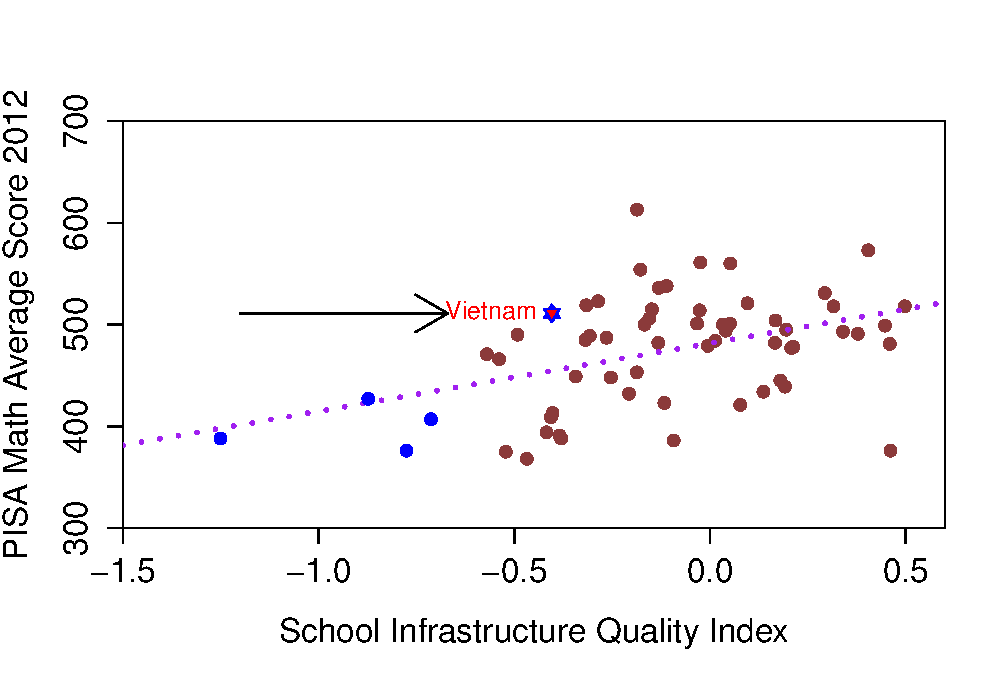
\includegraphics[width=0.75 \textwidth]{INTRFIG4.pdf} \\
\scriptsize{Source:OECD-PISA database        \hspace{3in}     }
   \label{Figure 1} 
\end{figure}


\section{Regression Approach II: Oaxaca-Blinder Decomposition} 

A key weakness of the Fryer-Levitt approach is that the pooled regression does not allow for regression coefficients to be different across countries. In this section, we set aside the Fryer-Levitt method to look at the data from a different analytical perspective. We use the Oaxaca-Blinder decomposition (OB) method, that has recently become quite popular for PISA analysis after the initial work by \cite{Ammermueller07} comparing the PISA results of Finland and Germany. 

\subsection{Overview of the OB Decomposition} 

The objective of OB is to decompose the mean differences. In this case it is the mean difference in Vietnam's PISA performance with each of the DEV7 countries individually. Extensions of OB allow for decompositions to be made throughout the distribution rather than only at the mean values, but we leave such an extension for further research regarding Vietnam's PISA performance. OB is based on a simple algebraic rearrangement of terms of the OLS regression of test scores. The mean outcome difference to be explained ($\Delta\bar{Y}$) is simply the difference of the mean outcomes for Vietnam and the comparison country. Let us denote the scores as $\bar{Y}_{V}$ and $\bar{Y}_{O}$, respectively:

\begin{equation}\label{differential}
\Delta \bar{Y} = \bar{Y}_{V} - \bar{Y}_{O}
\end{equation}

Now, as the OLS error terms are of mean zero by construction, (2) can be represented by

\begin{equation}\label{differential_2}
\Delta \bar{Y} = \boldsymbol{\bar{X}}_{V}'\boldsymbol{\hat{\beta}}_{V} - \boldsymbol{\bar{X}}_{O}'\boldsymbol{\hat{\beta}}_{O}
\end{equation}

\noindent In the twofold version of OB that we use in this paper, (3) can be represented either as 

\begin{equation}\label{vnref}
\Delta \bar{Y} = \underbrace{(\boldsymbol{\bar{X}}_{V} - \boldsymbol{\bar{X}}_{O})'  \boldsymbol{\hat{\beta}}_{V}}_\text{endowments} + \underbrace{\boldsymbol{\bar{X}}_{O}' (\boldsymbol{\hat{\beta}}_{V} - \boldsymbol{\hat{\beta}}_{O})}_\text{coefficients}
\end{equation}

\noindent or as

\begin{equation}\label{otherref}
\Delta \bar{Y} = \underbrace{(\boldsymbol{\bar{X}}_{V} - \boldsymbol{\bar{X}}_{O})'  \boldsymbol{\hat{\beta}}_{O}}_\text{endowments} + \underbrace{\boldsymbol{\bar{X}}_{V}' (\boldsymbol{\hat{\beta}}_{O} - \boldsymbol{\hat{\beta}}_{V})}_\text{coefficients}
\end{equation}

\noindent depending on which country is used as a reference country. We focus on this paper on the approach of (4), using Vietnam as the reference, and leave (5) and additional OB variations to subsequent research. 

We base the choice of regression specification on the findings so far. In line with per capita GDP of Vietnam compared with the Dev7 variables, there are a series of income level or wealth related variables for which Vietnam does poorly in comparison with Dev7. We term these variables WEALTH related variables. We include in it all variables for which Vietnam has poorer endowments, and the term WEALTH denotes that they have higher mean values in Dev7 countries, which are wealthier than Vietnam. These variables have typically not been included in the Fryer-Levitt regressions as they would have exacerbated rather than reduced the Vietnam gap. For example, the set includes mother's highest level of education, or MISCED, which is one ISCED level higher for Dev 7 as compared to Vietnam. A second set of variables, which we term as ED WEALTH are typically variables for which Vietnam does better and are good for education results. For instance, Vietnam has a higher level for PRESCHOOL and for time spent by students in mathematics lessons after school (OUTMATH). These two sets of variables together constitute the specification of the $\boldsymbol{X}_{V}$ and $\boldsymbol{X}_{O}$ vectors. 


Now it is an established result that the matrix decomposition reported in equation 8 also holds at the variable level, as the overall decomposition is nothing else but the sum of variable level decompositions \cite{Hlavac15}. We extend this notion further to look at aggregations by the two sets of variables - ED WEALTH and WEALTH. In the equations below, we have m variables in the EDWEALTH set and n variables in the WEALTH set: 

\begin{equation}
\underbrace{(\boldsymbol{\bar{X}}_{A} - \boldsymbol{\bar{X}}_{B})'  \boldsymbol{\hat{\beta}}_{R}}_\text{endowments}
 = \underbrace{\displaystyle \sum^m_{i=1}{(\bar{X}_{iV} - \bar{X}_{iO})\hat{\beta}_{iV}}}_\text{ ED WEALTH}
+ \underbrace{\displaystyle \sum^n_{i=1}{(\bar{X}_{iV} - \bar{X}_{iO})\hat{\beta}_{iV}}}_\text{WEALTH}
\end{equation}


\begin{equation}
\underbrace{\boldsymbol{\bar{X}}_{O}'(\boldsymbol{\beta_V}-\boldsymbol{\beta_O})  }_\text{coefficients}
 = \underbrace{\displaystyle \sum^m_{i=1}{\bar{X}_{iV}( \hat{\beta}_{OV}} - \hat{\beta}_{iV})}_\text{ ED WEALTH}
+ \underbrace{\displaystyle \sum^n_{i=1}{\bar{X}_{iV}( \hat{\beta}_{OV}} - \hat{\beta}_{iV})}_\text{WEALTH}
\end{equation}

\subsection{Findings from OB Decomposition} 

In Tables 13 through 15 we present the mathematics score findings from the OB decomposition for Vietnam compared with each of the Dev7 countries arranged by geographic area. We present the mean differences again between Vietnam and Dev7, then countries from Latin America (Colombia and Peru), Eastern Europe \& Central Asia (Albania), Middle East \& North Africa (Jordan and Tunisia), East Asia \& Pacific's (Indonesia and Thailand) as well as Shanghai. The number ``Sum Total ED WEALTH + WEALTH'' in the bottom row indicates the mean difference between Vietnam and each of the Dev7 countries. The top panel in each of Tables 13 through 15 presents the ED WEALTH variables - these are variables related to educational performance where Vietnam does better on mean values compared to the Dev7 countries. The lower panel in each of the tables presents the WEALTH variables - typically related to a country's income level, they are variables where the Dev7 countries do better. The paired column of numbers for each country indicates a hypothetical counter-factual. The `Endowments' column shows how much of the mean difference arises from a difference in the mean values, keeping the coefficients fixed at the level of Vietnam. The `Coefficients' column indicates how much of the difference is due to the difference in coefficients between Vietnam an the compared country, keeping the characteristics fixed at the mean level of the compared country. We begin the analysis by looking at Latin American countries Colombia and Peru in Table 13. 

	\begin{table}[H]
		\tiny
		\def\arraystretch{1}
		\def\tabcolsep{3}
		\centering
		\caption{OB Decomposition for mathematics: Sample Means and Latin America (Colombia and Peru)}
		\begin{threeparttable}
			\begin{tabular}{llrrrrrr}
				\toprule
				\midrule
				&       & \multicolumn{2}{c}{\textbf{Mean value}} & \multicolumn{2}{c}{\textbf{Colombia}} & \multicolumn{2}{c}{\textbf{Peru}} \\ 
				\cline{3-8} \\
				\scriptsize{\textbf{Category}}	 &  \scriptsize{\textbf{Variable Name}}     & \multicolumn{1}{c}{\textit{Dev 7 }} & \multicolumn{1}{c}{\textit{Vietnam}} & \multicolumn{1}{c}{\textit{Endowments}} & \multicolumn{1}{c}{\textit{Coefficients}} & \multicolumn{1}{c}{\textit{Endowments}} & \multicolumn{1}{c}{\textit{Coefficients}} \\
				\hline \\
				\textbf{} & INTERCEPT & \multicolumn{1}{c}{\textit{}} & \multicolumn{1}{c}{\textit{}} & \multicolumn{1}{c}{\textit{}} & 222.6017 & \multicolumn{1}{c}{\textit{}} & 247.8394 \\ \cline{2-8} 
				Students & PRESCHOOL & 0.7888 & 0.9120 & 0.1767 & \underline{21.2995} & 0.8096 & \underline{6.8201} \\[0.4em]
				& LATESCHOOL & 1.5131 & 1.1872 & 2.7914 & -7.0084 & 5.3749 & -6.8398 \\[0.4em]
				& NOREPEAT & 0.8085 & 0.9321 & 9.752 & 5.6154 & 5.1146 & 8.7662 \\[0.4em]
				& SHRS  & 3.7566 & 3.9597 & 2.1314 & 10.2102 & 2.56  & \underline{19.0496} \\[0.4em]\hline
				Parents & OUTMATH & 1.8280 & 3.1305 & \underline{6.3176} & \underline{13.8406} & 3.6561 & \underline{14.5438} \\[0.4em]
				& PARPRESSURE  & 0.2665 & 0.3837 & 5.2187 & 5.0041 & 1.9524 & \underline{4.8938} \\[0.4em]
				& TIGERMOM & 52.4472 & 62.4183 & 0.1958 & \underline{-14.0056} & -0.6088 & \underline{3.4834} \\[0.4em]
				& TEACHMOM & 12.1764 & 38.2821 & 2.0458 & 2.2844 & 1.4841 & \underline{3.9414} \\[0.4em]\hline
				Teachers & PROPCERT & 0.6757 & 0.7961 & -     & -     & -     & - \\[0.4em]
				& MATHPROFDEV & 40.5068 & 49.0086 & -0.2447 & -1.0775 & 0.0423 & -3.9528 \\[0.4em]
				& TCH\_INCENTV & -0.0317 & 0.2687 & 1.9205 & -0.4223 & 2.6139 & -1.3882 \\[0.4em]
				& TCM\_INSPE & 0.5882 & 0.8664 & \underline{-13.3928} & \underline{-0.5966} & -6.3926 & -11.6551 \\[0.4em]
				& TCM\_OBSER & 0.8015 & 0.9785 & \underline{-9.9929} & \underline{-5.2289} & -1.9658 & -37.8481 \\[0.4em]
				& COMP\_USE & 0.4345 & 0.6447 & -0.6  & 3.1921 & -0.3406 & 1.8251 \\[0.4em]
				& STU\_FEEDB & 0.7105 & 0.8419 & -0.3485 & \underline{-10.1593} & -0.6405 & 5.056 \\[0.4em]\hline
				Schools & EXC6\_MATHCOMP & 0.6268 & 0.8032 & -0.6487 & -8.5158 & 0.0019 & -10.8913 \\[0.4em]
				& SCMATBUI & -0.6322 & -0.3988 & -0.0363 & -0.4844 & -0.0379 & -0.7149 \\[0.4em]
				& SCL\_EXTR\_CL & 0.6538 & 0.9584 & \underline{-8.4506} & \underline{-9.4397} & -8.1854 & -11.5939 \\[0.4em]
				& SCORE\_PUBLIC & 0.3450 & 0.7567 & 2.6639 & 4.0431 & 7.0514 & 2.4778 \\[0.4em]\hline
				\\
				\scriptsize{\textbf{TOTAL	ED WEALTH}} &       &       &       & -0.5007 & 8.5509 & 12.4896 & -14.0269 \\   
				&       &       &       & 0\%    & 8\%   & 10\%     & -11\% \\ \hline 
				Students & EXAPPLM & 0.1111 & -0.2418 & 0.2362 & 1.6552 & 1.7418 & -0.0448 \\[0.4em]
				& EXPUREM & -0.1384 & 0.1587 & 2.9206 & 0.9846 & -0.0688 & -1.3801 \\[0.4em]
				& LHRS  & 3.5990 & 3.2207 & 9.528 & -44.012 & 14.0996 & -56.6772 \\[0.4em]
				& MHRS  & 3.8960 & 3.7878 & -3.6621 & 14.9222 & -4.8692 & 13.7176 \\[0.4em]\hline
				Parents & HISEI & 40.4196 & 26.6023 & -6.3504 & 7.3598 & -3.7414 & 3.6262 \\[0.4em]
				& MISCED & 3.1193 & 2.1744 & -2.143 & -1.2957 & -1.2325 & -10.9724 \\[0.4em]
				& WEALTH & -1.4606 & -2.1343 & 2.4134 & 17.4408 & 1.4103 & 17.2629 \\[0.4em]
				& CULTPOS & -0.1424 & -0.2361 & 0.3183 & 0.327 & 0.4633 & 1.8325 \\[0.4em]
				& HEDRES & -0.7427 & -1.0743 & -4.8774 & -7.6374 & -6.0766 & -3.1882 \\[0.4em]
				& BOOK\_N & 53.6393 & 50.7860 & -0.0504 & -5.2598 & 0.0089 & -6.5238 \\[0.4em]\hline
				Teachers & TXT\_BOOK & 0.7905 & 0.7855 & -5.6426 & -5.2097 & 0.629 & -14.3821 \\[0.4em]
				& CLSIZE & 35.0130 & 42.5043 & -0.5804 & -46.7664 & -9.4773 & -36.5348 \\[0.4em]
				& TCFOCST & 0.4975 & 0.1402 & 2.7312 & 0.8924 & 1.4043 & -0.7333 \\[0.4em]
				& TCMORALE & 0.0376 & -0.2941 & -7.7804 & 1.8946 & -1.9897 & -0.2643 \\[0.4em]
				& TCHPARTI & -0.2169 & -1.6445 & 6.7157 & 1.8929 & 14.9263 & -0.3443 \\[0.4em]\hline
				Schools & TOWN  & 0.4508 & 0.3101 & -3.0845 & -2.9438 & 1.4527 & -6.9018 \\[0.4em]
				& VILLAGE & 0.1403 & 0.4584 & -11.2676 & -1.7407 & -8.1092 & -1.6368 \\[0.4em]
				& PRIVATESCL & 0.1714 & 0.0832 & 4.4454 & -2.5786 & 10.9349 & -11.4833 \\[0.4em]
				& STU\_FEES & 25.7233 & 16.6104 & 4.5328 & -23.7404 & -     & - \\[0.4em]
				& RATCMP15 & 0.3909 & 0.2216 & 7.6894 & -12.933 & 3.6968 & -11.777 \\[0.4em]
				& SCHAUTON & -0.2542 & -1.0419 & -10.9579 & -0.3955 & -10.3639 & 0.5217 \\[0.4em]
				& EXC1\_BAND & 0.4710 & 0.1678 & 0.29099 & -2.4563 & -0.118 & 0.1559 \\[0.4em]
				\hline \\
				\scriptsize{\textbf{TOTAL	WEALTH}} &       &       &   & -14.57471 & -109.5998 & 4.7213 & -125.7274  \\   
				&       &       &       & -14\%    & -103\%    & 4\%     & -100\% \\ \hline
				\\
				\multicolumn{2}{l}{\scriptsize{\textbf{SUM TOTAL (ED WEALTH \& WEALTH)}}}   &      &  & \textbf{} & \textbf{106.4774} & \textbf{} & \textbf{125.2960}  \\
				&   &    &  & \textbf{} & \textbf{100\%} & & \textbf{100\%} &
				\bottomrule
			\end{tabular}
			\begin{tablenotes}[para,flushleft]
				Notes: The 'Mean values' for Dev7 and Vietnam are taken from the whole data set and represent the same values used for Section 2 - Endowment Differences. They are included here to reiterate the categorization of variables into WEALTH and ED WEALTH, depending on their comparative values between Dev7 and Vietnam. Underlined values represent those variables mentioned within the analysis.
			\end{tablenotes}
		\end{threeparttable}
		\label{tab:addlabel}%
	\end{table}%


The mean difference for Colombia is positive 106 points. Interestingly, differences on ED WEALTH endowments make a negligible contribution and the coefficients on ED WEALTH only account for positive 8\% of the difference. The endowments on WEALTH indicate a 14\% reduction for Colombia by adopting Vietnamese endowments, and a large 103\% reduction from coefficients.  The Colombia EDWEALTH coefficient column indicates some interesting results. While PRESCHOOL (students having attended PRESCHOOL) would have had a positive 21 point impact, note the negative 14 point impact on the variable called TIGERMOM (parents proactively following up with teacher regarding student's performance) and negative 10 point impact on STU\_FEEDB (teachers obtain written feedback from students). This might indicate that some of the features of countries are related to cultural factors that come together as a package - being a `Tiger Mom' may help the child in Vietnam, but perhaps not as much in Colombia!

A similar interpretation is possible regarding the variables TCM\_INSPE and TCM\_OBSERVER (teachers benefit from class room observation by external inspectors and principal/senior school staff) and SCL\_EXTR\_CL (extra classes at school). These have a negative value in the endowment column as well as the coefficients column. This means that if Colombian students had Vietnamese characteristics on these variables, the mean result for Colombia would have been lower than it already is. The interpretation would be that what is good for Vietnamese students, in a Vietnamese context as measured by PISA, may not be good for Colombian students. However, this finding should be taken with some caution as there are also some variables, like OUTMATH (time spent in extra classes for math outside of school) which have positive values on the endowments and the coefficients. 

Finally from Table 13 we can see that for Peru, ED WEALTH endowments make a positive 10\% contribution and the coefficients make a negative 11\% contribution. ED WEALTH variables that make a positive contribution in the coefficients column include PRESCHOOL, SHRS (hours of science instruction) and all the parent related variables. On the WEALTH endowments, there is a positive 4\% contribution and a negative 100\% contribution from coefficients. 

Table 14 presents data from the next three countries, Albania from the Eastern Europe \& Central Asia region and Jordan and Tunisia from the Middle East \& North Africa region.

	\begin{table}[H]
		\tiny
		\def\arraystretch{1}
		\def\tabcolsep{3}
		\centering
		\caption{OB Decomposition for mathematics: Eastern Europe \& Central Asia (Albania) and Middle East \& North Africa (Jordan and Tunisia)}
		\begin{threeparttable}
			\begin{tabular}{llrrrrrr}
				\toprule
				\midrule
				&       & \multicolumn{2}{c}{\textbf{Albania}} & \multicolumn{2}{c}{\textbf{Jordan}} & \multicolumn{2}{c}{\textbf{Tunisia}} \\
				\cline{3-8} \\
				\scriptsize{\textbf{Category}}	 &  \scriptsize{\textbf{Variable Name}}     & \multicolumn{1}{c}{\textit{Endowments}} & \multicolumn{1}{c}{\textit{Coefficients}} & \multicolumn{1}{c}{\textit{Endowments}} & \multicolumn{1}{c}{\textit{Coefficients}} & \multicolumn{1}{c}{\textit{Endowments}} & \multicolumn{1}{c}{\textit{Coefficients}} \\
				\hline \\
				\textbf{} & INTERCEPT & \multicolumn{1}{c}{\textit{}} & 100.7672 & \multicolumn{1}{c}{\textit{}} & 232.8262 & \multicolumn{1}{c}{\textit{}} & 220.3262 \\ \cline{2-8} 			
				Students & PRESCHOOL & 3.2606 & 14.9314 & 2.9304 & 8.8395 & 6.1004 & 8.8937 \\[0.4em]
				& LATESCHOOL & 2.5351 & -16.1377 & 4.0339 & \underline{-17.9123} & 5.1805 & \underline{-13.6441} \\[0.4em]
				& NOREPEAT & -1.1335 & 81.2394 & -0.5863 & -0.5305 & 11.7885 & \underline{-24.2972} \\[0.4em]
				& SHRS  & 8.103 & 18.4864 & -3.4578 & -1.8296 & 6.821 & 12.3146 \\[0.4em]\hline
				Parents & OUTMATH & 8.4386 & 5.9606 & 8.4886 & 12.3205 & 1.5262 & 12.4973 \\[0.4em]
				& PARPRESSURE  & 3.0612 & 6.3037 & 2.9216 & 8.3922 & 6.05  & -2.0319 \\[0.4em]
				& TIGERMOM & 0.0071 & -3.1614 & -1.456 & 0.7928 & -4.5979 & \underline{-4.6769} \\[0.4em]
				& TEACHMOM & 2.4287 & 4.431 & 2.0207 & 0.5374 & 3.4577 & -0.343 \\[0.4em]\hline
				Teachers & PROPCERT & -0.8449 & 6.3679 & -     & -     & 1.103 & -1.8785 \\[0.4em]
				& MATHPROFDEV & 0.0438 & -0.353 & 0.1404 & 0.0539 & -0.0296 & -5.3119 \\[0.4em]
				& TCH\_INCENTV & 3.4264 & -2.4877 & -0.3897 & 1.002 & 1.7686 & -0.8613 \\[0.4em]
				& TCM\_INSPE & -5.3929 & -17.0471 & 2.0905 & 4.5083 & 0.5072 & -16.981 \\[0.4em]
				& TCM\_OBSER & -     & -     & 0.0738 & \underline{-11.522} & -0.8747 & 8.2309 \\[0.4em]
				& COMP\_USE & -0.4169 & -0.3193 & 0.1317 & -6.769 & -1.3139 & 2.006 \\[0.4em]
				& STU\_FEEDB & -0.5089 & 7.7288 & -0.4144 & \underline{-4.888} & -1.645 & -0.1837 \\[0.4em]\hline
				Schools & EXC6\_MATHCOMP & 0.3129 & -9.663 & -0.8381 & \underline{-2.5399} & -1.3721 & -0.8139 \\[0.4em]
				& SCMATBUI & 0.388 & -4.8621 & 0.2473 & \underline{-3.7528} & 1.4125 & \underline{-13.0502} \\[0.4em]
				& SCL\_EXTR\_CL & -3.5828 & -2.9217 & -4.3968 & \underline{-9.0748} & -3.8009 & \underline{-17.7227} \\[0.4em]
				& SCORE\_PUBLIC & 5.3549 & 3.4256 & 5.9804 & 4.7486 & 7.2212 & -0.7671 \\[0.4em]\hline
				\\
				\scriptsize{\textbf{TOTAL	ED WEALTH}} &   &  25.4804 & 91.9218 & 17.5202 & -17.6237 & 39.3027 & -58.6209 \\   
				&       &  18\%     &   64\%    & 15\%    & -15\%    & 35\%     & -52\% \\ \hline 
				Students & EXAPPLM & 1.9364 & -0.5576 & 2.5477 & -1.9561 & -0.0268 & 0.7122 \\[0.4em]
				& EXPUREM & -0.2203 & 1.3971 & 2.1748 & 2.0725 & 3.0066 & 0.953 \\[0.4em]
				& LHRS  & -3.359 & -34.8084 & 15.7577 & \underline{-58.088} & 23.1941 & -63.0774 \\[0.4em]
				& MHRS  & 4.424 & 14.1238 & -0.1466 & 43.9865 & -3.834 & 24.3011 \\[0.4em]\hline
				Parents & \multicolumn{1}{l}{HISEI} & -     & -     & -     & -     & -4.5879 & -17.802 \\[0.4em]
				& MISCED & -5.6001 & 18.8463 & -5.2108 & -3.2033 & -0.8438 & 9.0345 \\[0.4em]
				& WEALTH & 0.4117 & -1.4204 & 1.5112 & 0.8037 & 0.8843 & 5.3532 \\[0.4em]
				& CULTPOS & 0.3533 & 0.5941 & -0.1767 & 0.9315 & -0.5056 & 0.2824 \\[0.4em]
				& HEDRES & -3.3855 & -5.5085 & -5.509 & -3.607 & -2.857 & -5.5976 \\[0.4em]
				& BOOK\_N & 0.0053 & -0.4736 & -0.2911 & -0.1599 & 0.1597 & 0.8503 \\[0.4em]\hline
				Teachers & TXT\_BOOK & -     & -     & 3.5046 & -16.7213 & 3.2614 & -33.4627 \\[0.4em]
				& CLSIZE & -8.6779 & -23.4445 & -5.4853 & -59.9741 & -8.5485 & 10.7592 \\[0.4em]
				& TCFOCST & 2.9242 & 0.3422 & 1.1106 & -0.8656 & -2.34511 & 1.3381 \\[0.4em]
				& TCMORALE & -6.2933 & -0.0748 & -0.4259 & -1.4027 & 3.9636 & 1.4813 \\[0.4em]
				& TCHPARTI & 11.3136 & 4.9119 & 0.5336 & 8.9057 & 3.4112 & 7.9172 \\[0.4em]\hline
				Schools & TOWN  & 5.0475 & -6.7474 & 2.5742 & -2.1225 & 6.7826 & 6.9162 \\[0.4em]
				& VILLAGE & -7.49 & -0.6774 & -10.417 & -1.5033 & -11.82 & 0.9214 \\[0.4em]
				& PRIVATESCL & -0.0055 & -0.0083 & 6.1701 & \underline{-12.8976} & -     & - \\[0.4em]
				& STU\_FEES & 0.671 & -10.8914 & -     & -     & -0.355 & -19.7408 \\[0.4em]
				& RATCMP15 & 2.9895 & -4.1902 & 3.8324 & \underline{-25.5703} & 1.8275 & -7.3367 \\[0.4em]
				& SCHAUTON & -4.4263 & -8.8247 & 1.6804 & 5.5624 & -2.7901 & -17.2538 \\[0.4em]
				& EXC1\_BAND & 0.5318 & -8.6246 & 0.0348 & -2.8344 & 0.154 & -3.1367 \\[0.4em]
				\hline \\
				\scriptsize{\textbf{TOTAL	WEALTH}} &    & -8.8496 & -66.0364 & 13.7697 & -128.6438 & 8.13119 & -96.5876  \\   
				&       &  -6\%  & -46\%  & 12\%    & -109\%    & 7\%     & -86\% \\ \hline
				\\
				\multicolumn{2}{l}{\scriptsize{\textbf{SUM TOTAL (ED WEALTH \& WEALTH)}}} &      & \textbf{143.2834} & \textbf{} & \textbf{117.8486} & \textbf{} & \textbf{112.5516}  \\
				&        &    & \textbf{100\%} & \textbf{} & \textbf{100\%} &   & \textbf{100\%} &
				\bottomrule
			\end{tabular}%
			\begin{tablenotes}[para,flushleft]
				Notes: The 'Mean values' for Dev7 and Vietnam are taken from the whole data set and represent the same values used for Section 2 - Endowment Differences. They are included here to reiterate the categorization of variables into WEALTH and ED WEALTH, depending on their comparative values between Dev7 and Vietnam. Underlined values represent those variables mentioned within the analysis.
			\end{tablenotes}
		\end{threeparttable}
		\label{tab:addlabel}%
	\end{table}%

Table 14 shows that the mean difference between Albania and Vietnam for mathematics was positive 143 points, the highest Vietnam advantage amongst all Dev7 countries. The OB decomposition indicates that if Albanian 15 year olds had Vietnamese endowments on ED WEALTH variables, their score would have been higher by 18\% and if they had Vietnam's coefficients on those variables, their score would have been higher by 64\%. Looking at the bottom panel, with Vietnam's WEALTH endowments, Albania's score would have been reduced by 6\% and with Vietnam's WEALTH coefficients while retaining its own characteristics would have lowered the score by 46\%. Interpretation needs to be made with care, for instance, a big boost would have come from the coefficient values on repetition, but this is probably driven by the rarity of repetition in Vietnam.

With Jordan, the gap to be explained is positive 118 points. On the ED WEALTH variables, endowment differences with Vietnam make for a positive 15\% contribution and the coefficients make for a negative 15\% contribution. Vietnamese endowments on ED WEALTH would make a reasonable contribution for Jordanian students, but the coefficients would pull in the opposite direction. Six variables contribute mainly to this negative direction - LATESCHOOL (number of times arriving late in the schoolday), TCM\_OBSER (teacher classroom observation by principal or senior school staff), STU\_FEEDB (written feedback from students for teacher), SCL\_EXTR\_CL, EXC6\_MATHCOMP (mathematics competition as extra-curricular activity) and SCMATBUI (index of quality of school infrastructure). On the WEALTH side, there is a positive 12\% contribution of endowments and a negative 109\% contribution of coefficients. The variables which contribute to this anomalous result include PRIVATESCL, LHRS (hours of language instruction) and RATCMP15 (available computers for 15 year olds). 

The mean difference for Tunisia is positive 113 points. Tunisia indicates the highest positive value of ED WEALTH endowments amongst all countries (35\%) and also the highest negative value on the coefficients (-52\%). The results for WEALTH for Tunisia indicate a positive 7\% contribution on endowments and a negative 86\% contribution on coefficients. The constituent variables have made their appearance in the previous commentary - for example, the contributions to the negative value on ED WEALTH coefficients for Tunisia come from LATESCHOOL (-13.6), NOREPEAT (-24.3), TIGERMOM (-4.6), SCMATBUI (-13.05), and SCL\_EXTR\_CL (-17.72).

Next, we turn to Table 15 which includes the remaining set of Dev7 countries from the East Asia \& Pacific's region - Thailand and Indonesia as well as the additional case of Shanghai, which has much better results even than Vietnam, and is included as an East Asian counterpoint to the Dev7 countries. 

\begin{table}[H]
	\tiny
	\def\arraystretch{1}
	\def\tabcolsep{3}
	\centering
	\caption{OB Decomposition for mathematics: East Asia \& Pacific's (Indonesia and Thailand) and Shanghai}
	\begin{threeparttable}
		\begin{tabular}{llrrrrrr}
			\toprule
			\midrule
			&       & \multicolumn{2}{c}{\textbf{Indonesia}} & \multicolumn{2}{c}{\textbf{Thailand}} & \multicolumn{2}{c}{\textbf{Shanghai}} \\
			\cline{3-8} \\
			\scriptsize{\textbf{Category}}	 &  \scriptsize{\textbf{Variable Name}}     & \multicolumn{1}{c}{\textit{Endowments}} & \multicolumn{1}{c}{\textit{Coefficients}} & \multicolumn{1}{c}{\textit{Endowments}} & \multicolumn{1}{c}{\textit{Coefficients}} & \multicolumn{1}{c}{\textit{Endowments}} & \multicolumn{1}{c}{\textit{Coefficients}} \\
			\hline \\
			\textbf{} & INTERCEPT & \multicolumn{1}{c}{\textit{}} & 181.3475 & \multicolumn{1}{c}{\textit{}} & 197.3024 & \multicolumn{1}{c}{\textit{}} & -88.5547 \\ \cline{2-8} 			
			Students & PRESCHOOL & \underline{6.2309} & \underline{6.0373} & -1.3537 & -17.271 & 1.0135 & 3.3683 \\[0.4em]
			& LATESCHOOL & 1.3545 & 0.1656 & 2.4103 & -6.5245 & -0.7333 & -9.4329 \\[0.4em]
			& NOREPEAT & 3.0327 & \underline{15.4797} & -0.8545 & 18.0457 & -2.4686 & 18.736 \\[0.4em]
			& SHRS  & 3.6461 & 3.2498 & -4.6096 & -1.3158 & 2.7618 & 11.5291 \\[0.4em]\hline
			Parents & OUTMATH & \underline{9.9458} & 3.9547 & 6.7928 & 12.3212 & 1.4415 & -19.6668 \\[0.4em]
			& PARPRESSURE  & 0.2358 & 7.19  & -1.4518 & 4.2812 & -3.295 & -2.5603 \\[0.4em]
			& TIGERMOM & -1.4622 & \underline{-5.0425} & -0.388 & -2.3087 & 1.7009 & -8.999 \\[0.4em]
			& TEACHMOM & 2.1566 & 1.7254 & 2.753 & 0.1281 & -4.4387 & 3.3083 \\[0.4em]\hline
			Teachers & PROPCERT & 1.0728 & \underline{7.8387} & -0.4727 & 31.4282 & 8.3337 & 43.4759 \\[0.4em]
			& MATHPROFDEV & -0.0778 & -4.2427 & 0.2289 & 0.5997 & 0.0199 & 0.5484 \\[0.4em]
			& TCH\_INCENTV & 0.2442 & 0.6929 & -0.3042 & 2.7973 & 0.3293 & 0.0993 \\[0.4em]
			& TCM\_INSPE & -1.7713 & -7.5635 & -6.9777 & -9.7581 & 0.4269 & 23.093 \\[0.4em]
			& TCM\_OBSER & -0.0742 & \underline{11.6516} & -0.0414 & 35.1591 & -0.0214 & -65.8268 \\[0.4em]
			& COMP\_USE & -0.6291 & 1.714 & 0.0932 & 3.2715 & 2.1571 & -3.3878 \\[0.4em]
			& STU\_FEEDB & 0.0796 & 7.9599 & -0.0804 & -3.4671 & 0.9525 & 15.1379 \\[0.4em]\hline
			Schools & EXC6\_MATHCOMP & -0.3133 & 1.5705 & -0.6327 & -15.9607 & -7.5785 & 46.1336 \\[0.4em]
			& SCMATBUI & 0.0048 & -1.1337 & 0.4918 & -0.3168 & 1.369 & -0.9102 \\[0.4em]
			& SCL\_EXTR\_CL & -2.9043 & \underline{-20.2148} & -0.299 & -31.4213 & -6.1388 & 29.4929 \\[0.4em]
			& SCORE\_PUBLIC & \underline{5.7895} & 1.2721 & 0.1084 & -1.5941 & -13.9127 & 6.2176 \\[0.4em]\hline
			\\
			\scriptsize{\textbf{TOTAL	ED WEALTH}} &   &  26.5611 & 32.305 & -4.5873 & 18.0939 & -18.0809 & 90.3565 \\   
			&       &  19\%     &   23\%    & -6\%    & 25\%    & -22\%     & 111\% \\ \hline 
			Students & EXAPPLM & 1.2618 & -0.0988 & 2.6597 & -0.6224 & -1.635 & 0.0304 \\[0.4em]
			& EXPUREM & 2.1991 & 0.1956 & 1.1331 & -0.244 & -0.0536 & -1.354 \\[0.4em]
			& LHRS  & -2.0941 & -29.3342 & -10.6968 & -28.5366 & -11.4368 & 1.8702 \\[0.4em]
			& MHRS  & 1.0459 & 14.6798 & 0.4215 & -18.4475 & 4.4884 & 7.1219 \\[0.4em]\hline
			Parents & \multicolumn{1}{l}{HISEI} & -1.7446 & -0.6415 & -3.7308 & 3.9065 & 8.6256 & 0.6227 \\[0.4em]
			& MISCED & -0.4967 & 6.245 & -1.5344 & -3.2852 & 2.0466 & 0.206 \\[0.4em]
			& WEALTH & -0.5319 & -1.6968 & 1.9975 & 4.6253 & -6.7778 & 6.9447 \\[0.4em]
			& CULTPOS & -0.3684 & 0.7266 & 0.2273 & -0.0479 & 2.4812 & -0.9197 \\[0.4em]
			& HEDRES & 2.5025 & -8.659 & -6.2788 & -2.0394 & 7.1149 & 2.2072 \\[0.4em]
			& BOOK\_N & -0.062 & 1.7571 & -0.3221 & -4.9515 & 5.1709 & 4.2595 \\[0.4em]\hline
			Teachers & TXT\_BOOK & 1.2766 & -17.5263 & 2.749 & -10.9737 & -2.4418 & 0.6483 \\[0.4em]
			& CLSIZE & -4.7921 & -13.5878 & -3.667 & -20.3239 & 0.4045 & 23.7015 \\[0.4em]
			& TCFOCST & 4.5553 & -4.0316 & 4.7078 & -9.8512 & 0.0868 & 0.7556 \\[0.4em]
			& TCMORALE & -9.9416 & 1.028 & -4.4468 & 1.0381 & 0.5319 & 2.9116 \\[0.4em]
			& TCHPARTI & 18.5498 & -10.6116 & 27.6836 & -19.9891 & -0.8565 & -11.9873 \\[0.4em]\hline
			Schools & TOWN  & 5.1411 & -1.5651 & 3.5728 & -3.3756 & -     & - \\[0.4em]
			& VILLAGE & -7.3432 & -1.496 & -9.3596 & -2.0706 & -     & - \\[0.4em]
			& PRIVATESCL & 2.0065 & 0.0116 & 0.1877 & 1.3994 & 1.9492 & 3.1875 \\[0.4em]
			& STU\_FEES & 11.4805 & -29.6824 & 0.2682 & -8.9641 & -0.1311 & 3.278 \\[0.4em]
			& RATCMP15 & -1.56 & -11.0681 & 7.5765 & -21.4644 & -3.1063 & 3.4899 \\[0.4em]
			& SCHAUTON & -17.2045 & 8.6425 & -21.8484 & 10.7935 & -7.8405 & 20.4172 \\[0.4em]
			& EXC1\_BAND & 0.4597 & -7.9357 & 0.6927 & 3.9018 & 24.6725 & 6.7965 \\[0.4em]
			\hline \\
			\scriptsize{\textbf{TOTAL	WEALTH}} &    & 4.3397 & -104.6487 & -8.0073 & -129.5225 & 23.2931 & 74.1877  \\   
			&       &  3\%  & -75\%  & -11\%    & -177\%    & 29\%     & 91\% \\ \hline
			\\
			\multicolumn{2}{l}{\scriptsize{\textbf{SUM TOTAL (ED WEALTH \& WEALTH)}}} &      & \textbf{139.9046} & \textbf{} & \textbf{73.2792} & \textbf{} & \textbf{81.2017}  \\
			&        &    & \textbf{100\%} & \textbf{} & \textbf{100\%} &   & \textbf{100\%} &
			\bottomrule
		\end{tabular}%
		\begin{tablenotes}[para,flushleft]
			Notes: The 'Mean values' for Dev7 and Vietnam are taken from the whole data set and represent the same values used for Section 2 - Endowment Differences. They are included here to reiterate the categorization of variables into WEALTH and ED WEALTH, depending on their comparative values between Dev7 and Vietnam. Underlined values represent those variables mentioned within the analysis.
		\end{tablenotes}
	\end{threeparttable}
	\label{tab:addlabel}%
\end{table}%

Table 15 indicates that in the case of Indonesia, the gap to be explained is positive 140 points. Endowments and coefficients on ED WEALTH account for positive 19\% and positive 23\% of the gap. The ED WEALTH variables explain more as was the case for Colombia. When we look at the WEALTH related variables, we see that the endowments of Indonesia would not have made such a big impact, pointing to the fact that Indonesia is closest to Vietnam amongst the Dev7 countries on per capita income. Of a similar magnitude like Colombia, we can see that the WEALTH coefficients of Vietnam would set back Indonesian students by negative 75\%.

Thailand is the country with the lowest difference in mathematics score, only positive 73 points behind Vietnam. The OB decomposition for Thailand indicates a negative 6\% contribution of endowments on EDWEALTH and a positive 25\% contribution on coefficients. On the WEALTH set of variables, the contribution for Thailand was negative 11\% on endowments and negative 177 \% on coefficients. The results from Shanghai, added to the mix as a counterpoint to Dev7 countries, do not seem to provide much additional insight. The biggest exlanation of difference between Vietnam and Shanghai would the coefficients on ED WEALTH and WEALTH, with 111\% and 91\% respectively. \footnote{For all other countries we used the respective country as the basis; For Shanghai, Vietnam is the base country in terms of equation (5)}. 

Overall, the OB decompositions support the previous findings. In five of the seven Dev7 countries, the ED WEALTH variables show a positive contribution on endowments - meaning that if the other countries have had Vietnam's endowments on ED WEALTH variables, their performance would have been better. On the coefficients side of ED WEALTH, we see a different picture - the contributions range from +64\% for Albania to -52\% for Tunisia, with other countries ranged in between. The two Asian countries (Indonesia and Thailand) have similar contributions of 23\% and 25\%. The predictable WEALTH set of decompositions is of less interest to us as in most cases there are small effects on endowments and large negative effects on coefficients. 

With cross-section data in a non-experimental context, it is very difficult to make definitive conclusions, and only tentative ones can be made that hint at some answers. The findings on Dev7 countries indicate that it is possible that a number of advantages that Vietnam enjoys, depicted in ED WEALTH, can only function effectively in combination. One way to consider this is through a cultural lens - meaning that there is something specific to Vietnamese culture, that enables Vietnam to benefit from hard working students and teachers, with the guidance of committed and involved parents, even in cities and small towns. 

\section{Conclusion}

This paper has sought to focus attention and find insights regarding a most remarkable PISA 2012 result - the superlative performance of Vietnam, a country with the lowest per capita income amongst all PISA participants. Vietnam, with a mean PISA math score of 511 is not one of the very top performers. However, when compared with other lower middle income countries that took part in PISA 2012, Vietnam is a clear outlier. The following three concluding points can be made as a result of the analysis presented in this paper.

\textbf{1. Half the gap can be explained:}  Even though the PISA dataset is rich and covers many aspects related to the achievement of student scores with international standardization of measures, with all the available variables, we could explain at best about 50\% of the performance gap of Vietnam. The PISA 2015 application will be especially interesting to study as it will provide another important data point and enable a trend analysis to be conducted. 

\textbf{2. Cultural factors are likely very important:} A combination of three sets of factors appear to be the most potent explanation for Vietnam's performance: First, Vietnamese students work harder - we see they have less instances of skipped classes and being late for school, spend about the same time or more learning in school and substantial extra time studying after school. While at school, Vietnamese students are more disciplined and focused on their studies. Second, Vietnamese teachers appear to benefit from a closer supervision of their work by the school principal and others, and there may be a stronger harmony between the hard working students and their teachers. Third, parents may have an important role to play, by taking an active part in combining high expectations of their children, following up with their children's teachers and contributing at school. 

\textbf{3. Resources do appear to matter:} When we compare PISA performances across the range from lower income non-OECD countries to the high income OECD countries, we find a clear positive trend. Vietnam has so far been the only PISA outlier, with a performance on par with much wealthier countries, and in fact one of the top performing countries in Science. The analysis indicates that Vietnam may be reaping the benefits of policies regarding investments in education - the most important factor probably being the higher level of access to pre-school. A second factor is the investment in school infrastructure, especially in cities and small towns.

The unique combination of focused educational investments beyond its income level and a cultural heritage that has positive behavioral implications for students appear to be part of the story behind Vietnam's educational success.

\newpage
\appendix
\begin{center}
\section*{Appendix}
\end{center}

\setcounter{table}{0}
\renewcommand{\thetable}{A\arabic{table}}


\begin{table}[H]
	\tiny
	\def\arraystretch{0.9}
	\centering
	\caption{Summary statistics - Additional variables used for regressions}
	\begin{threeparttable}
	\begin{tabulary}{1.0\textwidth}{L L C C C C}
		\hline\hline \\
		\multicolumn{2}{c}{}
		& \multicolumn{2}{c}{Dev7 countries}
		& \multicolumn{2}{c}{Vietnam}	\\
		\hline & & & & & & 
		Variable & Description & MS & Valid N &  MS & Valid N \\
		\hline \\
		ATSCHL \textit{(r)} & Attitude towards school - & 0.1616 & 25563 & 0.143 & 3246 \\
		& learning is useful & (0.9986) & &  (0.8648) \\ [0.3em]
		ATTLNACT \textit{(r)} & Attitude towards school - & 0.1233 & 25368 & -0.535 & 3248 \\
		& studying pays off & (0.964) & & (0.8212) & \\ [0.3em]
		TCHQUAL\_DIFF \textit{(r)} & with different teacher & 0.5249 & 24986 &  0.363 & 3231 \\
		& student would work harder & (0.4994) & & (0.481) & \\ [0.3em]
		BKGR\_FAMPROB \textit{(r)} & Problems at home & 0.4705 & 25038 & 0.264 & 3231 \\
		& deter effort in school & (0.4991) & & (0.4409) & \\ [0.3em]
		MTSUP \textit{(r)} & Mathematics supportive & 0.4778 & 25918 & 0.3685 & 3247 \\
		& teaching style & (0.9613) & & (0.774) & \\ [0.3em]
		TCHBEHTD \textit{(r)}& Teacher oriented & 0.4973 & 26433 & 0.2964 & 3254 \\ 
		& inctruction method & (1.0798) &  & (0.8099) &  \\ [0.3em]
		TCHBEHSO \textit{(r)} & Student oriented & 0.7921 & 26358 & 0.2969 & 3248 \\ 
		& instruction method & (0.9545) &  & (0.819) &  \\ [0.3em]
		TCHBEHFA \textit{(r)} & Assessment used to help &  0.4634 & 26245 & 0.005 & 3246 \\ 
		& students perform better & (0.9934) &  & (0.79) &  \\ [0.3em]
		TCSHORT & Shortage of & 0.4742 & 43144 & 0.418 & 4959 \\ 
		& teaching staff & (1.2601) &  & (1.1628) &  \\ [0.3em]
		TCFOCST & Teacher focus & 0.4932 & 43422 & 0.1321 & 4959 \\ 
		& & (1.0049) &  & (0.8347) &  \\ [0.3em]
		ST72Q01 \textit{(r)} & Class size & 31.0133 & 23946 & 41.0018 & 2735 \\ 
		& in 'test language' &  (9.3337) &  & (5.4001) &  \\[0.3em]
		LHRS \textit{(r)} & Learning time (hours per week) & 3.599 & 22177 & 3.2207 & 2870 \\
		& in 'test language' & (1.9887) & & (1.1576) & \\[0.3em]
		MHRS \textit{(r)} & Learning time (hours per week) & 3.896 & 21913 & 3.7878 & 2850 \\
		& in mathematics & (2.0335) & & (1.3764) & \\[0.3em]
		SHRS \textit{(r)} & Learning time (hours per week) & 3.7566 & 21701 & 3.9597 & 2473 \\
		& in science & (2.5078) & & (2.5484) & \\[0.3em]	
		\hline \\
		\multicolumn{6}{l}{\textbf{Quality assurance of mathematics teachers through ...}}	\\ [0.3em]
		\hline \\
		TCM\_STUASS & test or assessment & 0.8734 & 43048 & 0.9821 & 4959 \\ 
		& of student achievement & (0.3325) &  & (0.1328) &  \\ [0.3em]
		\hline \\
		\multicolumn{6}{l}{\textbf{Assessment used to}}	\\ [0.3em]
		\hline \\
		ASS\_PROG & inform parents & 0.9669 & 42703 & 0.9929 & 4959 \\ 
		& about childs progress & (0.179) &  & (0.0837) &  \\[0.3em] 
		ASS\_PROM & decide on students? & 0.8998 & 42478 & 0.9516 & 4959 \\ 
		& retention or promotion & (0.3002) &  & (0.2146) &  \\ [0.3em]
		ASS\_NAT & compare school to &  0.6951 & 42450 & 0.8804 & 4959 \\ 
		& national performance & (0.4604) &  & (0.3245) &  \\ [0.3em]
		ASS\_CUR & identify improvements & 0.8978 & 42475 & 0.9141 & 4959 \\ 
		& in the curriculum & (0.3029) &  & (0.2803) &  \\ [0.3em]
		\hline \\
		\multicolumn{6}{l}{\textbf{School policy related factors}}	\\ [0.3em]
		\hline \\
		EXC11\_UNICORN & School offers & 0.7108 & 41907 & 0.9635 & 4959 \\ 
		& 'country specific item' & (0.4534) &  & (0.1875) &  \\ [0.3em]
		LEADINST & Promotion of & 0.0732 & 43253 & -0.0465 & 4959 \\ 
		& instructional leadership & (1.0797) &  & (0.9424) &  \\ [0.3em]
		QUAL\_RECORD & Systematic recording of & 0.8824 & 42939 & 0.9821 & 4959 \\ 
		& data for quality assurance & (0.3221) &  & (0.1328) &  \\ [0.3em]
		SCHSEL & School selectivity/ & 2.3036 & 43296 & 2.8411 & 4959 \\ 
		& student admission policies & (0.7997) &  & (0.4074) &  \\ [0.3em]
		\hline	
	\end{tabulary}
		\begin{tablenotes}[para,flushleft]
		Notes: The variables relate to the questionnaires administered to schools and students in the rotated  
		booklet, marked with \textit{(r)}. For a more detailed description of variables, please see Tables A2, A3, A4 in the Appendix. The variable means of Dev7 and Vietnam are statistically different at the 95\% significance level, except ATTSCHL.Figures in parenthesis represent standard deviations. 
		\end{tablenotes}
		\end{threeparttable}
\end{table}


	\begin{table}[H]
		\tiny
		\def\arraystretch{0.9}
		\def\tabcolsep{4}
		\centering
		\caption{Variable overview - students variables}
		\begin{tabular}{llll}
			\toprule
			\midrule
			\textbf{Variable} & \textbf{Description} & \textbf{Questionnaire} & \textbf{Question reference} \\
			\midrule
			\\
			\textbf{STUDENTS} &       &       &  \\[0.4em]
			\\
			\multicolumn{4}{l}{\textbf{Student characteristics and family background (Table 1)}}  \\[0.4em] 
			\cline{1-4} \\    
			FEMALE & Sex of student & Student - general quest.  & ST04Q01 \\[0.4em]
			AGE   & Age of student & Student - general quest.  & OECD index \\[0.4em]
			PRESCHOOL & Attend Preschool (ISCED 0)  & Student - general quest.  & ST05Q01 \\[0.4em]
			REPEAT & Grade repeating & Student - general quest.  & OECD index \\[0.4em]
			ST08Q01/LATESCHOOL & Times late for school & Student - general quest.  & ST08Q01 \\[0.4em]
			ST09Q01 & Days unexcused absence & Student - general quest.  & ST09Q01 \\[0.4em]
			ST115Q01 & Times skipped classes & Student - general quest.  & ST115Q01 \\[0.4em]
			HISEI & Highest parental occupational status & Student - general quest.  & OECD index \\[0.4em]
			MISCED & Educational level of mother (ISCED) & Student - general quest.  & OECD index \\[0.4em]
			WEALTH & Family wealth possessions & Student - general quest.  & OECD index \\[0.4em]
			CULTPOS & Cultural possessions & Student - general quest.  & OECD index \\[0.4em]
			HEDRES & Home educational resources & Student - general quest.  & OECD index \\[0.4em]
			BOOK\_N & Number of books in family home & Student - general quest.  & OECD index \\[0.4em]
			\\
			\multicolumn{4}{l}{\textbf{Student effort (Table 2)}} \\[0.4em]
			\cline{1-4} \\  
			OUTMATH & weekly out-of-school lessons in math & Student - rotated quest. 2 & ST55Q02 \\[0.4em]
			OUTREAD & weekly out-of-school lessons in 'test language' & Student - rotated quest. 2 & ST55Q01 \\[0.4em]
			OUTSCIE & weekly out-of-school lessons in science & Student - rotated quest. 2 & ST55Q03 \\[0.4em]
			ST57Q01 & Out-of-school-time homework & Student - rotated quest. 2 & ST57Q01 \\[0.4em]
			ST57Q02 & Out-of-school-time guided homework & Student - rotated quest. 2 & ST57Q02 \\[0.4em]
			ST57Q03 & Out-of-school-time personal tutor & Student - rotated quest. 2 & ST57Q03 \\[0.4em]
			ST57Q04 & Out-of-school-time classes by company & Student - rotated quest. 2 & ST57Q04 \\[0.4em]
			ST57Q05 & Out-of-school-time parent/family member & Student - rotated quest. 2 & ST57Q05 \\[0.4em]
			ST57Q06 & Out-of-school-time learn on computer & Student - rotated quest. 2 & ST57Q06 \\[0.4em]
			\\
			\multicolumn{4}{l}{\textbf{Student attitude (Table 3)}} \\[0.4em]
			\cline{1-4} \\  
			MATWKETH & Mathematics work ethic & Student - rotated quest. 1 & OECD index \\[0.4em]
			SUBNORM & Subjective norms in mathematics & Student - rotated quest. 1 & OECD index \\[0.4em]
			OPENPS & Openness to problem solving & Student - rotated quest. 1 & OECD index \\[0.4em]
			SCMAT & Self-Concept of own math skills & Student - rotated quest. 3 & OECD index \\[0.4em]
			PERSEV & Perseverance in problem solving  & Student - rotated quest. 1 & OECD index \\[0.4em]
			ANXMAT & Mathematics anxiety & Student - rotated quest. 3 & OECD index \\[0.4em]
			MATINTFC & Mathematics intentions & Student - rotated quest. 1 & OECD index \\[0.4em]
			\\
			\multicolumn{4}{l}{\textbf{Student experience in mathematics (Table 4)}} \\[0.4em]
			\cline{1-4} \\  
			FAMCON & Familiarity with math concepts & Student - rotated quest. 2 & OECD index \\[0.4em]
			FAMCONC & FAMCON corrected with FOIL & Student - rotated quest. 2 & OECD index \\[0.4em]
			EXAPPLM & Experience with applied mathematics tasks at school & Student - rotated quest. 2 & OECD index \\[0.4em]
			EXPUREM & Experience with pure mathematics tasks at school & Student - rotated quest. 2 & OECD index \\[0.4em]
			\\
			\multicolumn{4}{l}{\textbf{Additional student variables used in regressions/decomposition (Table 13, 14, 15)}} \\[0.4em]     
			\cline{1-4} \\  
			NOREPEAT & 1 - REPEAT & Student - general quest.  & based on 'REPEAT' OECD index \\[0.4em]
			SHRS  & Learning time (hours per week) in science & Student - rotated quest. 2 & based on 'SMINS' OECD index \\[0.4em]
			LHRS  & Learning time (hours per week) in 'test language' & Student - rotated quest. 2 & based on 'LMINS' OECD index \\[0.4em]
			MHRS  & Learning time (hours per week) in mathematics & Student - rotated quest. 2 & based on 'MMINS' OECD index \\[0.4em]
			ATSCHL & Attitudes towards school - learning is useful & Student - rotated quest. 3 & OECD index \\[0.4em]
			ATTLNACT & Attitudes towards school - studying pays off & Student - rotated quest. 3 & OECD index \\[0.4em]
			BKGR\_FAMPROB & Problems at home deter effort in school & Student - rotated quest. 3 & ST91Q03 \\[0.4em]
			ST72Q01 & Class size in `test language' & Student - rotated quest. 3 & ST72Q01 \\[0.4em] 
			\bottomrule
			\multicolumn{4}{l}{Notes: For details on OECD indices, please see the PISA 2012 Technical Report \cite{OECD2014a}.}\\ 
		\end{tabular}%
		\label{tab:addlabel}%
	\end{table}%

	\begin{table}[H]
		\tiny
		\def\arraystretch{1}
		\def\tabcolsep{4}
		\centering
		\caption{Variable overview - parents and teachers variables}
		\begin{threeparttable}
		\begin{tabular}{llll}
			\toprule
			\midrule
			\textbf{Variable} & \textbf{Description} & \textbf{Questionnaire} & \textbf{Question reference} \\
			\midrule
			\\
			\textbf{PARENTS} &       &       &  \\[0.4em]
			\\
			\multicolumn{4}{l}{\textbf{Parental support at school (Table 5)}} \\[0.4em] 
			\cline{1-4} \\    
			PARPRESSURE & Parental achievement pressure & School questionnaire & SC24Q01 \\[0.4em] 
			TIGERMOM & Parent initiates - progress discussion & School questionnaire & SC25Q01, SC25Q03 \\[0.4em] 
			DUTYMOM & Teacher initiates - progress discussion & School questionnaire & SC25Q02, SC25Q04 \\[0.4em] 
			VOLUMOM & Parent participation - volunteering & School questionnaire & SC25Q05, SC25Q06, SC25Q07,  \\[0.4em] 
			&       &       & SC25Q09, SC25Q12 \\[0.4em] 
			TEACHMOM & Parent participation - teaching assistance & School questionnaire & SC25Q08 \\[0.4em] 
			FUNDMOM & Parent participation - fundraising & School questionnaire & SC25Q11 \\[0.4em] 
			COUNCILMOM & Parent participation - school government & School questionnaire & SC25Q10 \\[0.4em] 
			\\
			\textbf{TEACHERS} &       &       &  \\
			\\
			\multicolumn{4}{l}{\textbf{Teacher characteristics and management (Table 6)}}   \\[0.4em] 
			\cline{1-4} \\    
			PROPCERT & Proportion of certified teachers & School questionnaire & OECD index \\[0.4em] 
			SMRATIO & Mathematics teacher-student ratio & School questionnaire & OECD index \\[0.4em] 
			SC35Q02/MATHPROFDEV & Professional development in math in last 3 months & School questionnaire & SC35Q02 \\[0.4em] 
			STUDREL & Teacher student relations & Student - rotated quest. 3 & OECD index \\[0.4em] 
			TCH\_INCENTV & Teacher appraisal linked to incentives & School questionnaire & IRT index from SC31Q01-Q07 \\[0.4em] 
			TCH\_MENT & Teacher mentoring as quality assurance & School questionnaire & SC39Q08 \\[0.4em] 
			TCM\_PEER & Teacher peer review of elctures, methods etc & School questionnaire & SC30Q02 \\[0.4em] 
			TCM\_OBSER & Principal or senior staff observations & School questionnaire & SC30Q03 \\[0.4em] 
			TCM\_INSPE & Observation of classes external inspector & School questionnaire & SC30Q04 \\[0.4em] 
			\\
			\multicolumn{4}{l}{\textbf{Pedagogical practices (Table 7)}}  \\[0.4em]
			\cline{1-4} \\  
			COMP\_USE & Math policy - use of computers in class & School questionnaire & SC40Q01 \\[0.4em] 
			TXT\_BOOK & Math policy - same textbook  & School questionnaire & SC40Q02 \\[0.4em] 
			STD\_CUR & Maths policy - standardized curriculum & School questionnaire & SC40Q03 \\[0.4em] 
			ASS\_SCH & Formative assessment used to monitor  & School questionnaire & SC18Q05 \\[0.4em] 
			& the schools yearly progress  &       &  \\[0.4em] 
			ASS\_TCH & Formative assessment used to make  & School questionnaire & SC18Q06 \\[0.4em] 
			& judgements on teachers� effectiveness &       &  \\[0.4em] 
			COGACT & cognitive activation in mathematics lessons & Student - rotated quest. 3 & OECD index \\[0.4em] 
			STU\_FEEDB & Seeking written feedback from students & School questionnaire & SC39Q07 \\[0.4em] 
			CLSMAN & Teacher classroom management (in math) & Student - rotated quest. 3 & OECD index \\[0.4em] 
			DISCLIMA & Disciplinary climate in class (in math) & Student - rotated quest. 3 & OECD index \\[0.4em] 
			\\
			\multicolumn{4}{l}{\textbf{Additional teacher variables used in regressions/decomposition (Table 10, 11, 12, 13, 14, 15)}} \\[0.4em]
			\cline{1-4} \\  
			\multicolumn{4}{l}{\textit{Formative assessment used to ....}} \\[0.4em]
			ASS\_PROG & inform parents about childs progress & School questionnaire & SC18Q01 \\[0.4em]
			ASS\_PROM & decide on students retention or promotion & School questionnaire & SC18Q02 \\[0.4em]
			ASS\_NAT & compare school to national performance & School questionnaire & SC18Q04 \\[0.4em]
			ASS\_CUR & identify improvements in the curriculum & School questionnaire & SC18Q07 \\[0.4em]
			TCHBEHFA & help student perform better & Student - rotated quest. 3 & OECD index \\[0.4em]
			\bottomrule
			\end{tabular}%
			\begin{tablenotes}[para,flushleft]
			Notes: For details on OECD indices, please see the PISA 2012 Technical Report \cite{OECD2014a}.The same IRT approach was used to construct the TCH\_INCENTV index.
			\end{tablenotes}
			\end{threeparttable}
	\end{table}%

	\begin{table}[H]
		\tiny
		\def\arraystretch{1}
		\def\tabcolsep{4}
		\centering
		\caption{Variable overview - teachers variables continued, schools variables}
		\begin{tabular*}{1\linewidth}{@{\extracolsep{\fill}}llll}
			\toprule
			\midrule
			\textbf{Variable} & \textbf{Description} & \textbf{Questionnaire} & \textbf{Question reference} \\
			\midrule
			\\
			\textbf{TEACHERS cntd.} &       &       &  \\
			\\
			\multicolumn{4}{l}{\textbf{Additional teacher variables used in regressions/decomposition (Table 10, 11, 12, 13, 14, 15)}} \\[0.4em]
			\cline{1-4} \\ 	
			TCSHORT & Shortage of teaching staff & School questionnaire & OECD index \\[0.4em]
			TCFOCST & Teacher focus & School questionnaire & OECD index \\[0.4em]
			TCM\_STUASS & Test or assessment of student achievement & School questionnaire & SC30Q01 \\[0.4em]
			TCMORALE & Teacher morale & School questionnaire & OECD index \\[0.4em]
			TCHQUAL\_DIFF & different teacher student would work harder & Student - rotated quest. 3 & ST91Q04 \\[0.4em]
			MTSUP & Mathematics supportive teaching style & Student - rotated quest. 3 & OECD index \\[0.4em]
			TCHBEHTD & Teacher oriented instruction method & Student - rotated quest. 3 & OECD index \\[0.4em]
			TCHBEHSO & Student oriented instruction method & Student - rotated quest. 3 & OECD index \\[0.4em]
			\\
			\textbf{SCHOOLS} &       &       &  \\[0.4em]
			\\
			\multicolumn{4}{l}{\textbf{School characteristics (Table 8)}}  \\[0.4em] 
			\cline{1-4} \\    
			PRIVATESCL & Private school dummy variable & School questionnaire & SC01Q01 \\[0.4em]
			SC02Q02/STU\_FEES  & Funding from school from student fees  & School questionnaire & SC02Q02 \\[0.4em]
			VILLAGE  & School located in a village & School questionnaire & SC03Q01 \\[0.4em]
			TOWN  & School located in a town & School questionnaire & SC03Q01 \\[0.4em]
			CITY  & School located in a city & School questionnaire & SC03Q01 \\[0.4em]
			CLSIZE & Average class size & School questionnaire & OECD index \\[0.4em]
			SCHSIZE & Number of enrolled students at school & School questionnaire & OECD index \\[0.4em]
			PCGIRLS & Proportion of girls at school  & School questionnaire & OECD index \\[0.4em]
			\\
			\multicolumn{4}{l}{\textbf{School resources and management (Table 9)}}  \\[0.4em]
			\cline{1-4} \\  
			RATCMP15 & Available computers for 15-year-olds & School questionnaire & OECD index \\[0.4em]
			COMPWEB & Ratio of computers connected to internet & School questionnaire & OECD index \\[0.4em]
			SCMATEDU & Quality of school educational resources] & School questionnaire & OECD index \\[0.4em]
			SCMATBUI & Quality of physical infrastructure & School questionnaire & OECD index \\[0.4em]
			SCL\_EXTRA\_CL & School offers additional math classes & School questionnaire & SC20Q01 \\[0.4em]
			EXC1\_BAND & School offers band, orchstra or choir & School questionnaire & SC16Q01 \\[0.4em]
			EXC2\_PLAY & School offers school play/musical & School questionnaire & SC16Q02 \\[0.4em]
			EXC5\_MCLUB & School offers mathematics club & School questionnaire & SC16Q05 \\[0.4em]
			EXC6\_MATHCOMP & School offers mathematics competition & School questionnaire & SC16Q06 \\[0.4em]
			EXC10\_SPORT & School offers sporting activities & School questionnaire & SC16Q10 \\[0.4em]
			SCORE\_PUBLIC & Achievement data posted publicly & School questionnaire & SC19Q01 \\[0.4em]
			SCORE\_AUTHRITS & Achievement data tracked by authority & School questionnaire & SC19Q02 \\[0.4em]
			SCHAUTON & School autonomy in admininistrative decisions & School questionnaire & OECD index \\[0.4em]
			TCHPARTI & Teacher participation in administrative decisions & School questionnaire & OECD index \\[0.4em]
			LEADCOM & Communicating and acting on defined school goals & School questionnaire & OECD index \\[0.4em]
			STUDCLIM & Student-related aspects of school climate & School questionnaire & OECD index \\[0.4em]
			TEACCLIM & Teacher-related aspects of school climate & School questionnaire & OECD index \\[0.4em]
			\\
			\multicolumn{4}{l}{\textbf{Additional school variables used in regressions/decomposition (Table 10, 11, 12, 13, 14, 15)}}  \\[0.4em]
			\cline{1-4} \\  
			EXC11\_UNICORN & School offers 'country specific item' & School questionnaire & SC16Q11 \\[0.4em]
			LEADINST & Promotion of instructional leadership & School questionnaire & OECD index \\[0.4em]
			QUAL\_RECORD & Systematic recording of data for quality assurance & School questionnaire & SC39Q03 \\[0.4em]
			SCHSEL & School selectivity/student admission policies & School questionnaire & OECD index \\[0.4em]
			\bottomrule
			\multicolumn{4}{l}{Notes: For details on OECD indices, please see the PISA 2012 Technical Report \cite{OECD2014a}.}\\
		\end{tabular*}%
		\label{tab:addlabel}%
	\end{table}%



\newpage
\begin{thebibliography}{9} %

\bibitem[Ammermueller, 2007]{Ammermueller07}
Andreas Ammermueller,
``PISA: What makes the difference? Explaining the gap in test scores between   
Finland and Germany'',
\emph{Empirical Economics}, 2007, 33:263�287

\bibitem[Barnett, 1995]{Barnett95}
W.Steven Barnett,
``Long-Term Outcomes of Early Childhood Programs'',
\emph{The Future of Children}, 1995, 5(3):25-50

\bibitem[Blinder, 1973]{Blinder73}
Alan S. Blinder,
``Wage Discrimination: Reduced Form and Structural Estimates'', \emph{Journal of  
	Human Resources}, 1973, 8(4):436-455.

\bibitem[Chua, 2011]{Chua11}
Amy Chua, 
\textit{Battle Hymn of the Tiger Mother}, Penguin Press, New York, 2011 

\bibitem[Dalton and Ong, 2005]{DaltonOng05}
Russell J.Dalton and Nhu-Ngoc T.Ong,
``Authority Orientations and Democratic Attitudes: A Test of the �Asian Values�
Hypothesis'', \emph{Japanese Journal of Political Science}, 2005, 6(2):1-21

\bibitem[Dang, 2007]{Hai-Anh07}
Hai-Anh Dang,
``The determinants and impact of private tutoring classes in Vietnam'',
\emph{Economics of Education Review}, 2007, 26:684�699

\bibitem[Fryer and Levitt, 2004]{FryerLevitt04}
Roland G. Fryer Jr. and Steven D.Levitt,
``Understanding the Black-White Test Score Gap in the First Two Years of School'',
\emph{The Review of Economics and Statistics}, May 2004, 86 (2):447-464

\bibitem[Ha and Harpham, 2005]{HaHapharm05}
Tran Thu Ha and Trudy Harpham,
``Primary education in Vietnam: Extra classes and
outcomes'', \emph{International Education Journal}, 2005, 6(5):626-634

\bibitem[Hlavac, 2015]{Hlavac15}
Marek Hlavac,
``oaxaca: Blinder-Oaxaca Decomposition in R'', R package version 0.1.2., \href{http://CRAN.R-project.org/package=oaxaca}{R package: oaxaca} 

\bibitem[Hsin and Xie, 2014]{HsinXie14} 
Amy Hsin and Yu Xie,
``Explaining Asian Americans� academic advantage over whites'',
\emph{Proceedings of the National Academy of Sciences}, May 2014,
111 (23) 8416-8421, \href{http://www.pnas.org/cgi/doi/10.1073/pnas.1406402111}{Hsin and Xie, PNAS 2014}

\bibitem[Lamport, 1994]{lamport94}
   Leslie Lamport,
   ``\emph{\LaTeX:} a document preparation system'', Addison Wesley, Massachusetts, 2nd edition, 1994

\bibitem[Tuan Anh Le, 2007]{Le07}
Tuan Anh Le,
``Applying realistic mathematics education in Vietnam : teaching middle school geometry'', Doctoral Dissertation, Universit\"at Potsdam, 2007,  
\href{https://publishup.uni-potsdam.de/opus4-ubp/frontdoor/index/index/year/2007/docId/1232}{Doctoral dissertation Tuan Le 2007} 

\bibitem[Danh Nam Nguyen and Trung Tran, 2013]{NguyenTran13}
Danh Nam Nguyen and Trung Tran,
``Recommendations for Mathematics Curriculum Development in Vietnam'',
Proceedings of the 6th International Conference on Educational Reform (ICER 2013): ASEAN Education in the 21st Century, \href{https://www.researchgate.net/publication/263077203_Recommendations_for_mathematics_curriculum_development_in_Vietnam}{Conference Paper, 2013}

\bibitem[Oaxaca, 1973]{Oaxaca73}
Ronald L. Oaxaca,
``Male-Female Wage Differentials in Urban Labor Markets'', \emph{International 
	Economic Review}, 1973, 14(3):693-709.

\bibitem[OECD, 2013a]{OECD2013a}
OECD, ``PISA 2012 Results: Excellence Through Equity: Giving Every 
Student the Chance to Succeed (Volume II)'', OECD Publishing, 2013,
\href{http://www.oecd.org/pisa/keyfindings/pisa-2012-results-volume-ii.htm}{OECD PISA 2012 Results Volume II}

\bibitem[OECD, 2014a]{OECD2014a}
OECD, ``PISA 2012 Technical Report'', OECD Publishing, 2014,
\href{http://www.oecd.org/pisa/pisaproducts/pisa2012technicalreport.htm}{OECD PISA 2012 Technical Report}

\bibitem[Vu Dinh Phuong, 2014]{Phuong14}
Vu Dinh Phuong,
``Using Video Study to Investigate Eighth-grade Mathematics Classrooms in Vietnam'', Doctoral Dissertation, Universit\"at Potsdam, 2014,
\href{https://publishup.uni-potsdam.de/frontdoor/index/index/docId/6999}{Doctoral Dissertation Vu Dinh Phuong 2014}

\bibitem[Schweinhart et al, 2005]{Schweinhartetal05}
Lawrence J. Schweinhart, Jeanne Montie, Zongping Xiang, W. Steven Barnett, Clive R. Belfield, and Milagros Nores,
``Lifetime Effects: The High/Scope Perry Preschool Study Through Age 40'', \emph{Monographs of the High/Scope Educational Research Foundation, 14}, Ypsilanti, MI: High/Scope Press, 2005


\end{thebibliography}



\end{document}
